%!TEX root = ../thesis.tex

\thispagestyle{myheadings}

\graphicspath{{Body/Figures/TrackingFigures/}{Body/Figures/TrackingFigures/OriginalDocumentationPlots/}{Body/Figures/TrackingFigures/OriginalDocumentationPlots/PlanePlots/}{Body/Figures/TrackingFigures/OriginalDocumentationPlots/PullPlots/}{Body/Figures/TrackingFigures/OriginalDocumentationPlots/Residuals/}{Body/Figures/TrackingFigures/eLossAndMaterial/}{Body/Figures/TrackingFigures/CoordSys/}{Body/Figures/TrackingFigures/TrackerPics/}{Body/Figures/TrackingFigures/Field/}{Body/Figures/TrackingFigures/TrackingFlow/}{Body/Figures/TrackingFigures/LeftRight/}{Body/Figures/TrackingFigures/Misc/}{Body/Figures/TrackingFigures/Extrapolation/}{Body/Figures/TrackingFigures/Tracks/}{Body/Figures/TrackingFigures/BeamMeasurements/}{Body/Figures/TrackingFigures/MCDataComparison/}{Body/Figures/TrackingFigures/VacuumPlots/}{Body/Figures/TrackingFigures/UpdatedDocumentationPlots/Images/}{Body/Figures/TrackingFigures/VacuumPlots/}{Body/Figures/TrackingFigures/Feb19DataPlots/Images/}}

\chapter{Track Reconstruction and Analysis}
\label{chapter:TrackReconstruction}

As described in section \ref{sec:StrawTrackers}, the straw trackers are used to provide information about the muon beam, important for the calorimeter \wa analysis, calculating the \wa pitch correction, and determining the spatially weighted magnetic field seen by the muons. The track reconstruction is performed in three stages: First, individual hits in the tracker are grouped into individual tracks in the finding stage. Second, a best trajectory is fit to grouped hits in the fitting stage. Third, the best fit trajectory is extrapolated back to the storage region or forwards to the calorimeter in the extrapolation stage. A fourth refinement stage is planned but not yet implemented, which would add or remove hits in the finding stage based on the results of the fitting and extrapolation stages.

As a brief aside, every stage of the track reconstruction is performed in the event-processing framework known as \textit{art} \cite{art}. The \textit{art} framework is a collection of modularized stages in a C++ framework useful for reading, reconstructing, filtering, analyzing, and writing data, among other things. All Fermilab experiments now use \textit{art}, and E989 is no exception.


\section{Track finding}
\label{sec:TrackFinding}

The track finding stage consists of pattern recognition routines in order to group individual hits into separate sets corresponding to individual incident tracks. The general implementation of these pattern recognition routines is relatively straightforward \cite{trackfinding,trackfinding2}. Hits across all modules are grouped in time windows called time islands, with an average width of $\SI{40}{ns}$ and a max width of $\SI{100}{ns}$. Within those time islands hits are then grouped into clusters. Clusters consist of one or two hits for each U or V view per module. As a reminder the U and V views of a module consist of the two U or V layers in that module, \secref{sec:StrawTrackers}. Hits are only clustered if they lie in close proximity in time and space to one another. The spatial constraint is defined as the difference in hit straw numbers, from 0 to 31 for the 32 straws per layer, which by default is limited to less than or equal to 4. Neighboring hit clusters in the same module are then grouped to form seeds, one per module. Finally, seeds in successive modules are grouped starting from one end of the tracker to form what are called track candidates. The seeds are formed and grouped into track candidates again only if they lie close in time and space to one another. The entire track candidate formation process occurs for all hits in a time island to find as many real tracks as possible. See \figref{fig:TrackCandidateSelection}.

After a track candidate has been formed a number of checks are made before passing it on to the fitting stage. If hits, clusters, or seeds are found to be shared among multiple track candidates, the candidates are dropped. Likewise, a track candidate is dropped if it is made from seeds consisting of only one type of view, or if the track candidate has less than six hits. There are also various small geometry and timing algorithms to improve the track candidates, such as removing hits from secondaries \cite{trackfinding3}. The $t_{0}$ time for the track candidate is calculated as the mean time of all hits, with some fixed offset at the end. This $t_{0}$ is helpfully constrained by geometry effects, where for a straight track passing through two layers in the same view, the sum of the drift times adds up to a constant (cite or show this?). The track candidate is supplied with an original momentum and position guess at the start of the track by fitting a circle to the hit straw wires in the horizontal plane. The final track candidates are passed on to the fitting stage. 


\begin{figure}[]
    \centering
    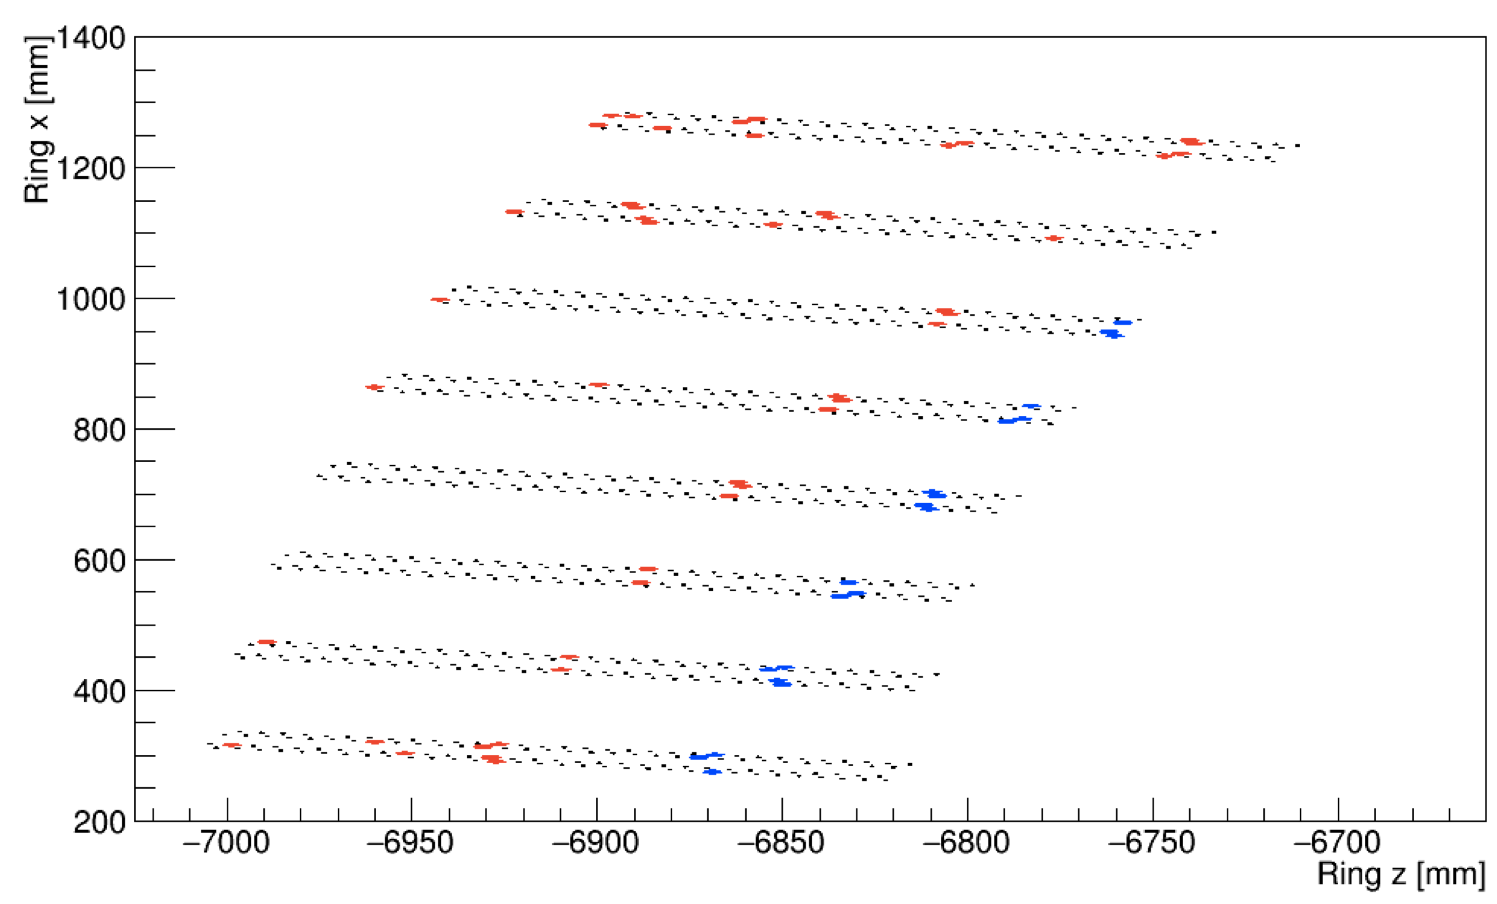
\includegraphics[width=0.9\textwidth]{TrackCandidateSelection}
    \caption[Track candidate selection]{Hits in a tracker station in a single time island. The black dots indicate the position of the straws, while the blue and red points indicate hits. In blue is the first formed track candidate in the island, formed from separate seeds in different modules. The track finding algorithms will move onto the remaining hits in the time island to attempt to form other track candidates, one of which is easily observable by eye.}    
    \label{fig:TrackCandidateSelection}
\end{figure}

% event display tracks

% \begin{figure}[]
% 	\centering
% 	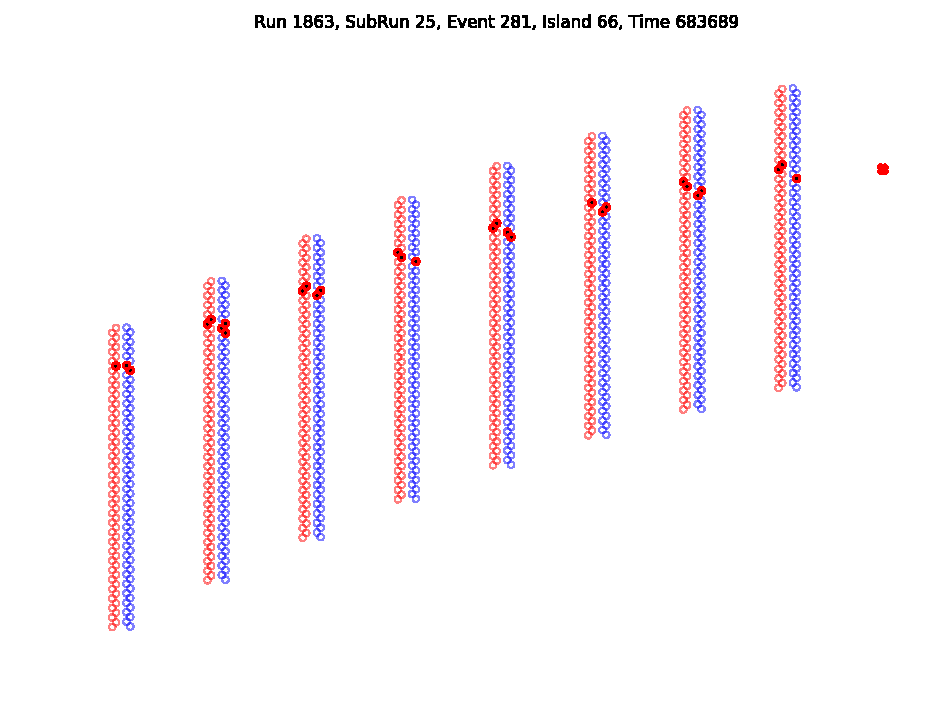
\includegraphics[width=0.9\textwidth]{TrackAndCaloHit}
%     \caption[TrackAndCaloHit]{clean up and possibly replace}    
%     \label{fig:TrackAndCaloHit}
% \end{figure}

% \begin{figure}[]
% 	\centering
% 	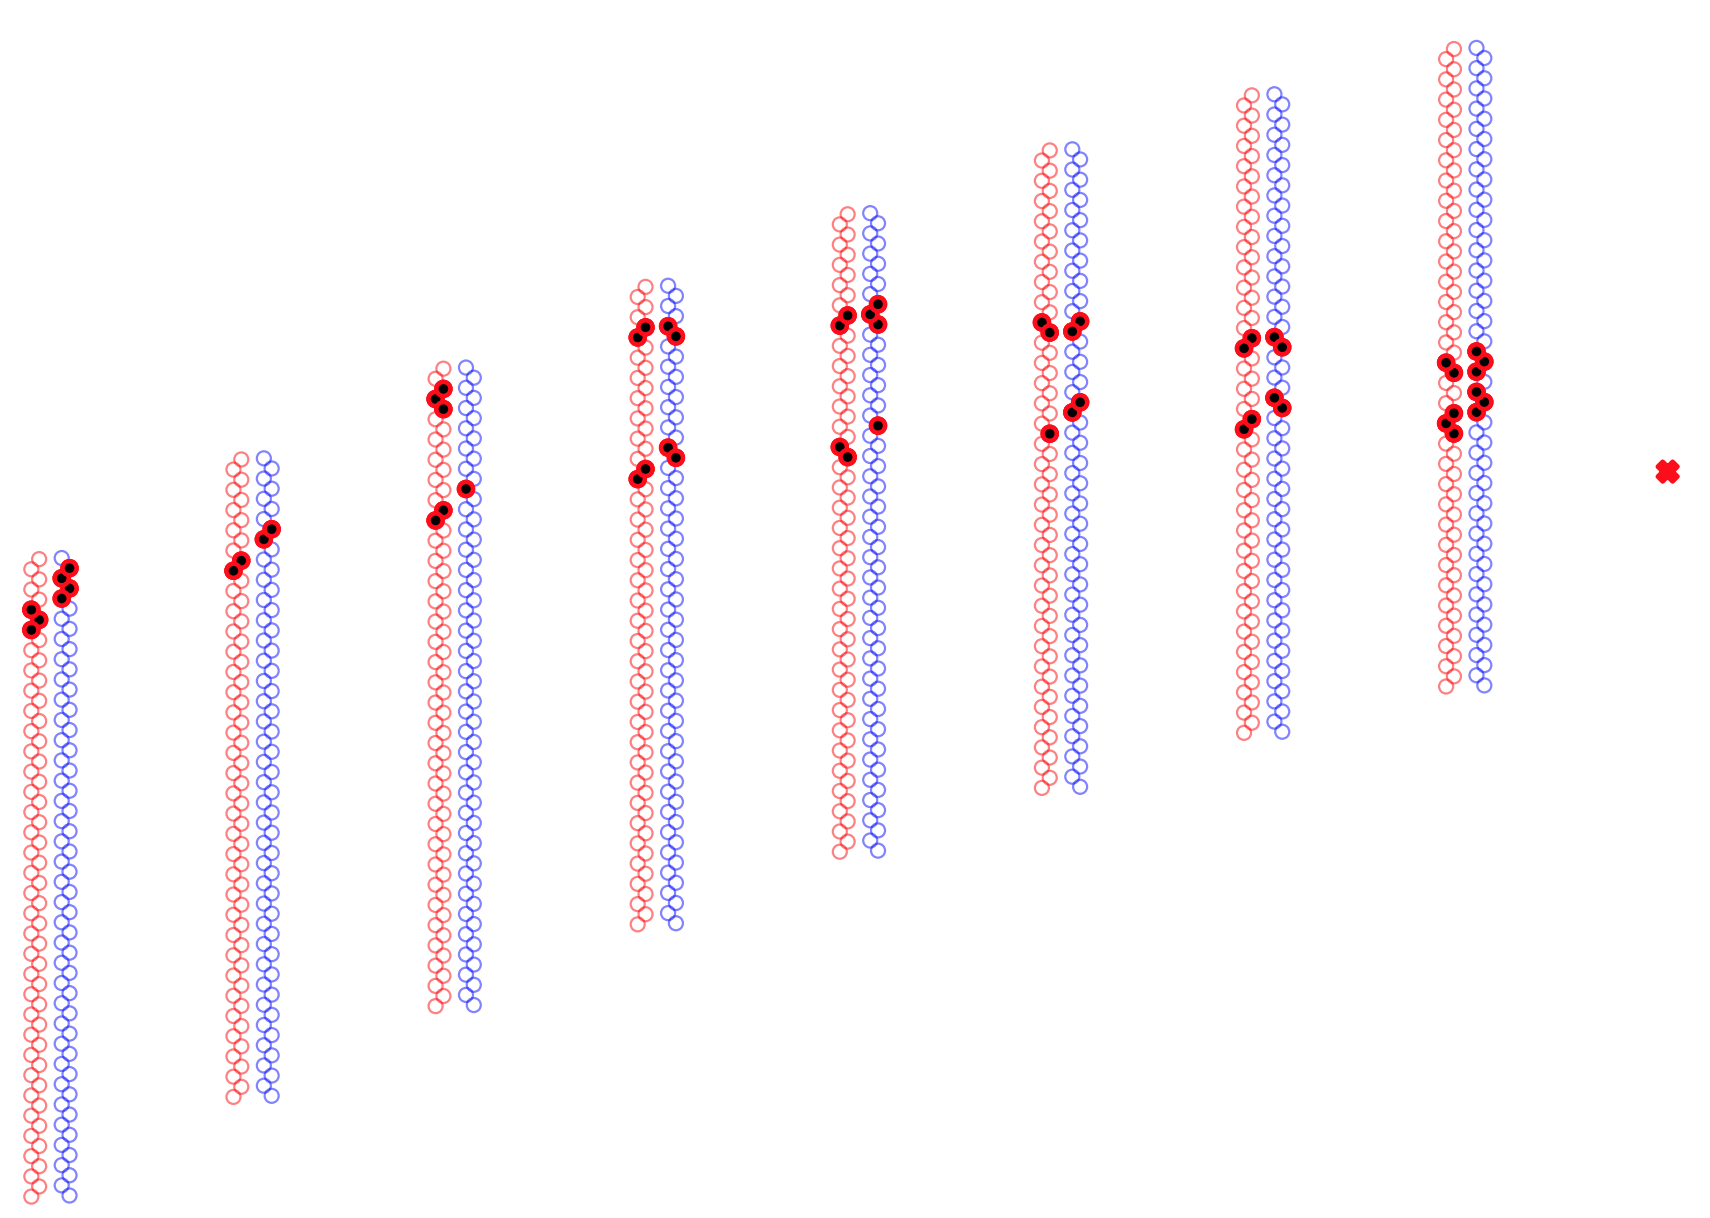
\includegraphics[width=0.9\textwidth]{pileupEvent}
%     \caption[pileupEvent]{clean up and possibly replace}    
%     \label{fig:pileupEvent}
% \end{figure}



\section{Track fitting}
\label{sec:TrackFitting}


The track fitting stage takes the track candidates from the track finding stage, and outputs a best fit trajectory to those candidates. This includes optimal state vectors and error matrices for the track at each measurement plane and at a ficticious starting plane at the entrance to the straw tracking detector. The track fitting routines can roughly be split into two parts, error propagation and the actual fitting and improvement of the track. The implementation of these parts go hand in hand, and will be described in turn. Details of the track fitting code itself is described in \refref{trackfittingdoc}. 


\subsection{Error propagation and coordinate systems}
\label{sub:Geane}

To put it simply, the process of error propagation involves taking track parameters and error matrices (which describe the spread in those track parameters) and transporting them along discrete steps from one point to another, accounting for changes due to any present magnetic fields or material along the step path. There is a set of error propagation routines originally written in Fortran by the EMC collaboration, called ``Geometry and Error Propagation'' or Geane \cite{geanemanual}. Geane works by propagating particles along their average trajectories neglecting the effects of discrete processes, using a helix equation along small enough steps where the change in the magnetic field is small. These routines were used in the E821 experiment as well as the PANDA and FINUDA experiments with some success \cite{Lavezzi}. The Geane routines were at one point converted to C++ and added to Geant4. The strength of using Geane within a Geant4 simulation lies in its direct access to the Geant4 geometry and field. This is crucially important for the E989 track fitting because the trackers live in a region of high field non-uniformity. Shown in \figref{fig:Opera2DFields} is the location of the tracker with respect to the radial and vertical fields. As shown the radial field in the tracker region rises from $\SI{0}{T}$ at the outer ends to roughly $\SI{.3}{T}$ at the inner top and bottom ends, and the vertical field drops approximately 50\% from the storage dipole field of $\SI{1.451}{T}$. These large field gradients over the tracking measurement space must be handled appropriately, which Geane does nicely.



\begin{figure}[]
\centering
    \begin{subfigure}[]{0.75\textwidth}
        \centering
        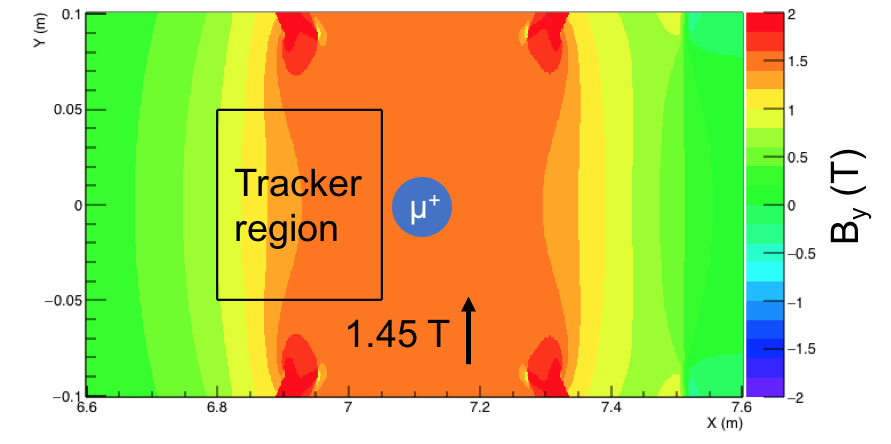
\includegraphics[width=\textwidth]{operaByMod}
        \caption{Vertical magnetic field}
    \label{fig:operaBy}
    \end{subfigure}%
    \vspace{5mm}
    \begin{subfigure}[]{0.75\textwidth}
        \centering
        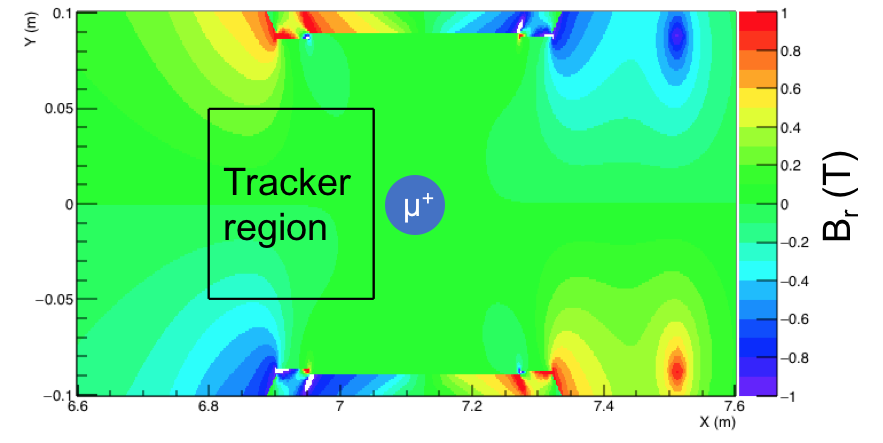
\includegraphics[width=\textwidth]{operaBxMod}
        \caption{Radial magnetic field}
    \label{fig:operaBx}
    \end{subfigure}
\caption[Vertical and radial magnetic fields calculated in Opera2D]{Shown are the vertical (top) and radial (bottom) magnetic fields of the storage ring magnet in and around the storage region as calculated in Opera 2D. The horizontal and vertical axes are the radial and vertical coordinates of the ring respectively. The center of the storage region lies at $\SI{7.112}{m}$ along the horizontal axis. The contours represent the strengths of the vertical and radial magnetic fields. The black box shows the rough location of the tracker with respect to the ring. It can be seen that there is a large field non-uniformity within the tracker space.}
\label{fig:Opera2DFields}
\end{figure}


Predicted track parameters in Geane are a function of path length 
        \begin{align} \label{eq:pp}
            p_{l} = F_{l,l_{0}}(p_{0}),
        \end{align}
where $p_{0}$ are some original tracker parameters and $p_{l}$ are the updated ones. The path length $l$ can be defined or limited how one wishes, and typically corresponds to a single step in the Geant4 simulation. The track parameter vectors $p$ are defined in some coordinate system. In the Geane routines these track parameters are $5 \times 1$ vectors either defined in the ``free'' (curvilinear) system
        \begin{align}
            \frac{1}{p}, \lambda, \phi, y_{\perp}, z_{\perp},
        \end{align}
or the ``surface'' (detector) system 
        \begin{align} \label{eq:UVW}
            \frac{1}{p}, \frac{p_{v}}{p_{u}}, \frac{p_{w}}{p_{u}}, v, w.
        \end{align}
In the free system, the $\lambda$ and $\phi$ parameters are the dip $(\pi/2 - \theta)$ and azimuthal angles respectively, while the $y_{\perp}$ and $z_{\perp}$ parameters are defined as being in the $XY$ or $XZ$ global Geant4 planes and orthogonal to $x_{\perp}$, where $x_{\perp}$ is defined as being along the momentum vector of the particle. See \figref{fig:FreeSurfaceSystems}. In the surface system, the UVW coordinates are defined with any two orthogonal vectors V and W\footnote{For clarification, the UVW surface system has nothing to do with the UV orientations of the straws at this time.}. The surface system is most usefully defined in the tracker reference frame, where the modules are staggered in a local Z coordinate, the local Y coordinate is vertical, and the local X coordinate increases with straw number. See \figref{fig:trackerReferenceFrame}. The surface system is then defined as
        \begin{align}
            \frac{1}{p}, \frac{p_{x}}{p_{z}}, \frac{p_{y}}{p_{z}}, x, y.
        \end{align}
In both free and surface systems the track is represented by one momentum parameter, two directional parameters, and two position parameters. Needing six independent parameters to describe a particle in space and momentum (three momentum and three position parameters), one parameter is left out and taken as a known variable. For Geane this is taken either as a known path length in the free system, or a known U coordinate in the surface system (or known Z coordinate in our tracker reference frame). In our tracker reference frame, the 32 straw layers corresponding to a tracking station are defined at known local Z coordinates. The path lengths for steps in Geane can be set to be equal to the distance for a track to travel between between detector planes, and therefore the track parameter dependence on the path length can instead by replaced by a dependence on plane number. The number of degrees of freedom per track is the number of measurements planes it hits, $N$, minus 5 for the number of track parameters.

\begin{figure}[]
  \centering
  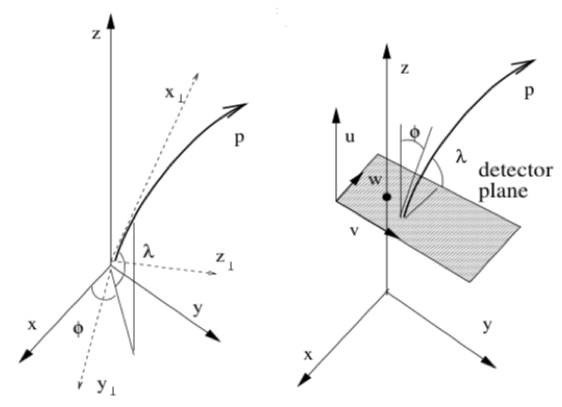
\includegraphics[width=0.5\textwidth]{FreeSurfaceSystems}
    \caption[Free and surface tracking coordinate systems]{Free (left) and surface (right) tracking coordinate systems.}
    \label{fig:FreeSurfaceSystems}
\end{figure}

\begin{figure}[]
  \centering
  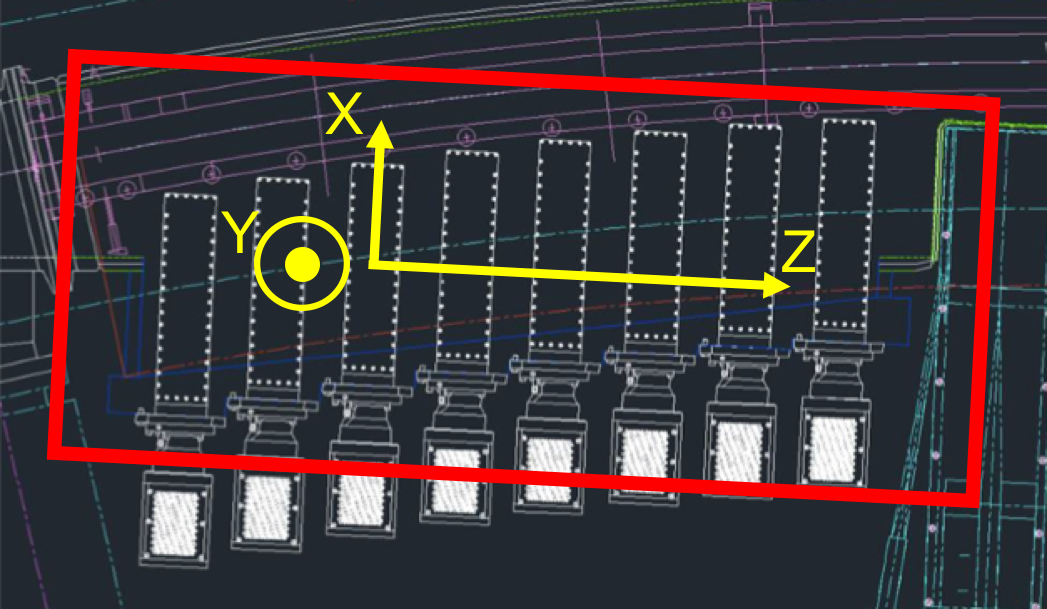
\includegraphics[width=0.7\textwidth]{trackerReferenceFrame}
    \caption[Tracker reference frame]{Shown is a model view of a tracker station in relation to the magnetic ring. Tracker modules are shown in white. Around the tracker measurement area is defined a coordinate system called the tracker reference frame. In that frame, the X coordinate is directed outward along the straws nearly radially, the Y coordinate is directed vertically up, and the Z coordinate is directed along the direction that the tracker modules are staggered.}
    \label{fig:trackerReferenceFrame}
\end{figure}


The $5 \times 5$ error matrix on a plane calculated in Geane describing the expected distribution in true parameters about the average ones is defined as
    \begin{align} \label{eq:errormatrix}
        \sigma_{N}^{ij} = <p_{N}^{i}p_{N}^{j}> - <p_{N}^{i}> \cdot <p_{N}^{j}>,
    \end{align} 
where i and j are track parameter indices and $N$ is some plane number. This error matrix will include effects from multiple scattering, delta ray production, ionization, and bremsstrahlung \cite{geanemanual,Lavezzi,energyloss}. These matrices are transported from plane to plane by what are called transport matrices, where the $5 \times 5$ transport matrix elements between two planes are defined as 
    \begin{align} \label{eq:transportmatrix}
        T_{N,N-1}^{i,j} = \frac{\partial p^{i}_{N}}{\partial p^{j}_{N-1}}.
    \end{align}
The transport matrix $T$ is a Jacobian between planes which expresses the infinitesimal changes in parameters at some plane (or path length) with respect to the parameters at some previous plane (or previous path length):
    \begin{align} \label{eq:parametertransport}
        \delta p_{N} &= T_{N,N-1} \delta p_{N-1}
    \end{align}
Note that the transport matrix does not propagate the track parameters themselves as with an equation of motion. The error matrix is propagated forward from one plane to another by
    \begin{align} \label{eq:errortransport}
        \sigma_{N} &= T_{N,N-1} \sigma_{N-1} T_{N,N-1}^{T} + \sigma_{\text{material}},
    \end{align}
where $\sigma_{\text{material}}$ is the added error due to material effects between the planes. See \figref{fig:FittingMatricesDiagram}. The calculation of the transport matrices themselves is done within the Geane routines in the free system on a step by step basis, where the derivation of the transport matrix elements is given in \refref{jacob}. It should briefly be pointed out that the transport matrix between any two planes (or number of steps) is the multiple of all intermediate transport matrices,
    \begin{align}
        T_{N,N-2} = T_{N,N-1} T_{N-1,N-2},
    \end{align}
regardless of what reference system the matrices are defined in (as long as they are all consistent). Geane can convert the transport matrices between the free system and the surface system using further Jacobians, also derived in \refref{jacob}. When converting a transport matrix from one reference system to another,
    \begin{align} \label{eq:Ttransform}
        T_{N,N-1}^{s} = A_{N} T_{N,N-1}^{f} A_{N-1}^{-1},
    \end{align}
where the $s$ and $f$ superscripts stand for the surface and free reference systems respectively, and $A$ is the Jacobian between reference frames which is defined at a specific point or plane $(A_{N} \neq A_{N-1})$. The error matrices are converted between reference frames in the usual way, 
    \begin{align} \label{eq:Sigtransform}
        \sigma_{N}^{s} &= A_{N} \sigma_{N}^{f} A_{N}^{T}.
    \end{align}


\begin{figure}[]
  \centering
  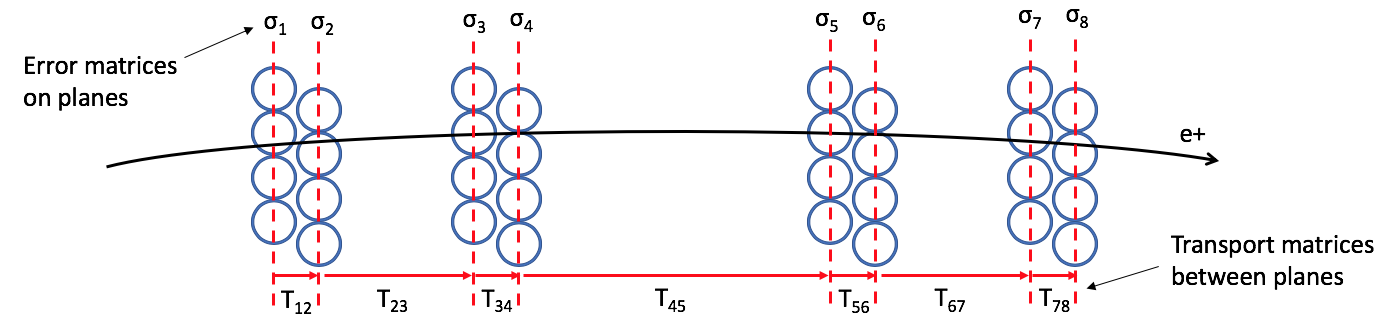
\includegraphics[width=\textwidth]{FittingMatricesDiagram}
    \caption[Transport and error matrices for straw tracker planes]{Transport matrices are defined between straw planes, and error matrices are defined on the planes.}
    \label{fig:FittingMatricesDiagram}
\end{figure}



Finally, while the tracker reference frame is nominally defined in the local XYZ coordinates as described previously, the straws themselves don't measure in that frame directly. As described in \secref{sec:StrawTrackers}, the straws measure drift circles in planes perpendicular to the straws themselves. The measurements from U and V straws therefore lie on the U and V measurement axes shown in \figref{fig:GeaneCoordSys}, where the measurement of the drift circle is instead taken as a U or V coordinate to the left or right of the straw wire. To first order the U or V coordinate is the DCA of the hit, which can be corrected with the angle of the track to get a better estimate, as shown in \appref{app:angularcorrection}. It's important to note that out of the five track parameters each straw only measures only a single U or V position. The new coordinate system is defined as
        \begin{align} \label{eq:trackermeasurementframe}
            \frac{1}{p}, \frac{p_{u}}{p_{z}}, \frac{p_{v}}{p_{z}}, u, v,
        \end{align}
where this $Z$ variable is the tracker reference frame $Z$, and the U and V coordinates here are non-orthogonal and are different to those in \equref{eq:UVW}. The transformation between the $XYZ$ and $UVZ$ systems is given by
    \begin{align}
        p^{UV} &= J_{5} p^{XY} \\
    \end{align}
where $J_{5}$ is a $5 \times 5$ matrix defined by
        \begin{align}
            J_{5} = 
            \begin{pmatrix}
                1 & 0 & 0 \\
                0 & J_{2} & 0 \\
                0 & 0 & J_{2}
            \end{pmatrix}
        \end{align}
and $J_{2}$ is a $2 \times 2$ matrix given by
        \begin{align}
            \begin{pmatrix}
                u \\
                v \\
            \end{pmatrix} =
            J_{2}
            \begin{pmatrix}
                x \\
                y \\
            \end{pmatrix} =
            \begin{pmatrix}
                \cos{\theta} & -\sin{\theta} \\
                \cos{\theta} & \sin{\theta} \\
            \end{pmatrix}
            \begin{pmatrix}
                x \\
                y \\
            \end{pmatrix}.
        \end{align}
$J_{2}$ is easily determined from \figref{fig:GeaneCoordSys}. In order to transform the transport or error matrices from the tracker reference frame to the tracker measurement frame, the same relations as in Equations~\ref{eq:Ttransform} and \ref{eq:Sigtransform} apply,
    \begin{align}
        T_{N,N-1}^{UV} &= J_{5} T_{N,N-1}^{XY} J_{5}^{-1} \\
        \sigma_{N}^{UV} &= J_{5} \sigma_{N}^{XY} J_{5}^{T}
    \end{align}
where the superscripts of $XY$ or $UV$ identify which coordinate system the objects belong to.

\begin{figure}[]
  \centering
  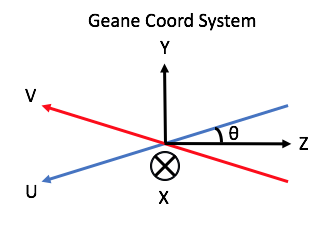
\includegraphics[width=0.5\textwidth]{GeaneCoordSys}
    \caption[Natural tracker measurement system]{The straw tracker measurement reference system. The XYZ system here is the straw tracker reference frame. $\theta$ is the same angle as the stereo angle of the straws, at 7.5\textdegree{}. U straws measure along the U axis and V straws measure along the V axis.}
    \label{fig:GeaneCoordSys}
\end{figure}




\subsection{\texorpdfstring{\chisq}{chisq} minimization}
\label{sec:TrackFittingAlgorithm}


The method for fitting and improving the track is a global \chisq minimization algorithm that uses the transport and error matrices as described previously \cite{geanemanual,trajfit}. This straightforward global fitting algorithm works because of the minimal amount of material contained within the tracker and the resulting small correlations between planes. For denser detectors with greater correlations, other fitting algorithms such as a Kalman filter should be used \cite{Lavezzi}. The following derivations and minimization assume measurements on planes in the tracker measurement frame described by \equref{eq:trackermeasurementframe}, but it should be noted that the results apply to any reference frame. A derivation for a \chisq including no material correlations is presented followed by one which includes said correlations.


The $\chi^{2}$ for a track is defined as the residuals between predicted and measured parameters on a measurement plane, divided by their errors, summed over all hit planes:
    \begin{align} \label{eq:chi2sum}
        \chi^2 = \sum_{i=1}^{N} [(p_{i}(p_{s})-x_{i})^{T} (\sigma_{i}^{-1}) (p_{i}(p_{s})-x_{i})]
    \end{align}
$x_{i}$ are vectors of the measured track parameters on plane $i$, $p_{i}$ are vectors of the average predicted track parameters which stem from some general starting parameters $p_{s}$, and $\sigma_{i}$ are the $5 \times 5$ error matrices on the plane\footnote{The vector $p_{s}$ has no numerical value at this time.}. To first order the error matrices consist only of the measurement errors on the U and V parameters and exclude the effects of random material processes. These errors are located in the U and V diagonal elements $(3,3)$ and $(4,4)$ respectively, with corresponding resolutions of \mum{150} as described in \secref{sec:StrawTrackers}. At second order the material error matrices as calculated by Geane are added to the measurement errors. Because the measured parameters consist of solely U or V measurements, the $x_{i}$ vectors are $5 \times 1$ objects where only the $(3)$ or $(4)$ elements have any meaning respectively\footnote{A straw tracker module as a whole can be approximated as measuring in 2D space, but this leads to correlations between measured parameters which must be taken into account, as compared to the natural tracker measurement frame in 1D space of U or V for which there are no measurement correlations \cite{UVcorrelations}. A fitting algorithm which fits the true measurement space of the drift circles themselves would be even better.}. The errors on the non-measured parameters in the diagonals of the error matrix are taken as infinite, such that when the error matrix is inverted all corresponding rows and columns of the final matrix on each plane reduce to zero and contribute nothing to the $\chi^{2}$.


By minimizing this \chisq with respect to the starting parameters $p_{s}$, and evaluating it at the target best starting guesses $p'_{0}$, which are the parameters of interest, the track can be fit:
    \begin{equation}
    \begin{aligned}
        \frac{\partial \chi^{2}}{\partial p_{s}}\Big|_{p_{s}=p'_{0}} = 0 
            &= \sum_{i=1}^{N}\Big[ \Big(\frac{\partial p_{i}(p_{s})}{\partial p_{s}}\Big|_{p_{s}=p'_{0}}\Big)^{T} (\sigma_{i}^{-1}) (p_{i}(p'_{0})-x_{i}) \\ 
            &+ (p_{i}(p'_{0})-x_{i})^{T} \Big(\frac{\partial(\sigma_{i}^{-1})}{\partial p_{s}}\Big|_{p=p'_{0}}\Big) (p_{i}(p'_{0})-x_{i}) \\ 
            &+  (p_{i}(p'_{0})-x_{i})^{T} (\sigma_{i}^{-1}) \Big(\frac{\partial p_{i}(p_{s})}{\partial p_{s}}\Big|_{p_{s}=p'_{0}}\Big)\Big]
    \label{eq:chi2summinimize}
    \end{aligned}
    \end{equation}
The middle term is small and can be neglected assuming that that the error matrix doesn't change much with respect to the choice of starting parameters. This is true as the error matrix is already small due to the low amount of material in the tracker. (In tandem the error matrix doesn't change much from one fitting iteration to the next as long as the path length through the material remains about the same.) The first and third terms are identical in value, and so must therefore both separately be equal to zero. \equref{eq:chi2summinimize} is therefore reduced to 
    \begin{align} \label{eq:chi2sumreduced}
        0 = \sum_{i=1}^{N} T^{T}_{i0} \sigma_{i}^{-1} (p_{i}(p'_{0})-x_{i}),
    \end{align}
where $T_{i0}$ is the transport matrix between the point at which the starting parameters are defined and plane $i$ given by \equref{eq:transportmatrix}:
    \begin{align} \label{eq:transportfrom0}
         T_{i0} = \frac{\partial p_{i}(p_{s})}{\partial p_{s}}\Big|_{p_{s}=p'_{0}}
    \end{align}
In minimizing the \chisq the desire is to update some original set of starting track parameters $p_{0}$ to the new best ones $p'_{0}$. This difference, $\Delta p_{0}$, can be determined by substituting the following equation into \equref{eq:chi2sumreduced},
    \begin{align} \label{eq:psub}
        p_{i}(p'_{0}) = p_{i}(p_{0}) + T_{i0} \Delta p_{0},
    \end{align}
which follows from \equref{eq:parametertransport}. After simplifying one arrives at 
    \begin{align} \label{eq:deltap}
        \Delta p_{0} = \sigma_{p_{0}} \sum_{i=1}^{N} T^{T}_{i0}(\sigma_{i}^{-1})(x_{i} - p_{i}(p_{0})),
    \end{align}
where
    \begin{align} \label{eq:cov}
        \sigma_{p_{0}} = [\sum_{i=1}^{N} T^{T}_{i0} (\sigma_{i}^{-1}) T_{i0} ]^{-1}.
    \end{align}
$\sigma_{p_{0}}$ is a $5 \times 5$ covariance matrix of the starting fit parameters, where the diagonals describe the fit errors in the 5 track parameters at that point. 
% \footnote{It should be noted that this minimization procedure does not supply the fit errors on each of the measurement planes, and only does so at the starting plane of the track.}

To summarize, an initial set of starting parameters $p_{0}$ are propagated forwards in Geane to produce predicted track parameters, transport matrices, and error matrices. These objects along with the measured parameters are plugged into the \chisq minimization algorithm detailed here to provide a \chisq describing the goodness of the fit corresponding to those original starting parameters, an improvement $\Delta p_{0}$ to those starting track parameters, and the errors $\sigma_{p_{0}}$ on those starting parameters. This consists of a single iteration of the track fitting. In order to determine the predicted parameters of the track corresponding to the improved starting parameters, the procedure needs to be repeated. The track fitting is iterated until the \chisq no longer improves, at which point the track fitting is said to have converged. Typically three or four iterations are enough to get a best fit track, as shown in \figref{fig:Iterations}. As a reminder the initial set of starting parameters is given by a circle fit to the hit straws as described at the end of \secref{sec:TrackFinding}. The starting parameters for a track are defined on a virtual $0$ plane parallel to the measurement planes, where the placement of the $0$ plane is defined based on a track by track basis and is placed at a point $\SI{1}{cm}$ in front of the first straw tracker module that was hit. Note that there is remarkable robustness with respect to the initial starting parameters in fitting the track. Of course if the initial starting parameters are too poor, then the fit will not converge. 


\subsection{Fits to idealized tracks in vacuum}


The tracking algorithm was first built and tested in a toy Monte-Carlo Geant4 simulation, and then ported over to the full \gmtwo simulation in \textit{art}. In the initial tests of the track fitting material was turned off and the measured hits were defined as the truth hits with some known smearing. (The truth hits are accessible within the Geant4 simulation by defined ``dummy plane'' detectors which record hits at the straw measurement planes.) Plots showing the goodness-of-fit for the fitted tracks are shown in \figref{fig:VacuumGoodnessOfFit}. Beyond the goodness-of-fit plots, the other measure of how good the track fitting is performing is to plot the truth pulls of the fit parameters. The truth pulls are defined as the residual between the fitted parameter and the truth parameter, divided by the fit error on that parameter:
    \begin{align}
        \frac{\Delta p^{i}_{0}}{\sigma_{p_{0}}^{ii}} = \frac{p^{i}_{0, \text{fit}} - p^{i}_{0, \text{true}}}{\sigma_{p_{0}}^{ii}}
    \end{align}
Since the \chisq minimization returns fit parameters and errors on the starting plane, this is where the truth pulls are defined. Plots of the truth pulls for the five track parameters are shown in \figref{fig:VacuumTruthPulls}, where each pull is a unit Gaussian as they should be for idealized results.


% By turning the material off, any scattering effects are eliminated which might affect the \chisq and fitted track. By taking the measured hits as truth hits, and dependence on which side of the wire the track went is removed. % This last bit is weird to say now since I haven't really talked about the left-right stuff yet.

    \begin{figure}[]
    \centering
        \begin{subfigure}[t]{0.45\textwidth}
            \centering
            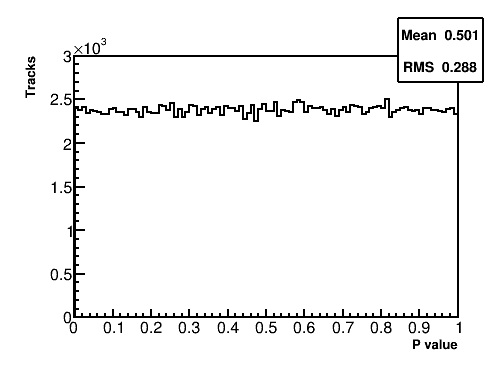
\includegraphics[width=\textwidth]{Vacuum_Pvalue}
            \caption{P value distribution for all tracks.}
        \end{subfigure}
        \begin{subfigure}[t]{0.45\textwidth}
            \centering
            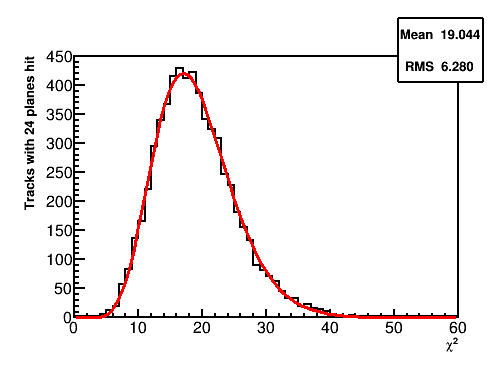
\includegraphics[width=\textwidth]{Vacuum_Chi2}
            \caption{\chisq distribution for tracks which hit 24 planes.}
        \end{subfigure}
    \caption[P value and \chisq distribution for fitted tracks in vacuum]{Goodness-of-fit distributions for fitted tracks in vacuum, with no material effects. The P value distribution is flat, and the \chisq distribution matches a normalized \chisq pdf for 19 degrees of freedom which is overlayed in red. (\chisq distributions for tracks which hit other numbers of planes are very similar.) Only tracks which have failed due to Geant4 reasons are excluded.}
    \label{fig:VacuumGoodnessOfFit}
    \end{figure}

    \begin{figure}[]
    \centering
        \begin{subfigure}[t]{0.45\textwidth}
            \centering
            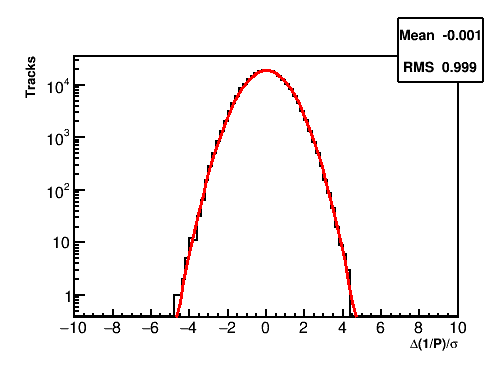
\includegraphics[width=\textwidth]{Vacuum_TruthPull_1P}
            \caption{$1/P$}
        \end{subfigure}%

        \vspace{2mm}
        \begin{subfigure}[t]{0.45\textwidth}
            \centering
            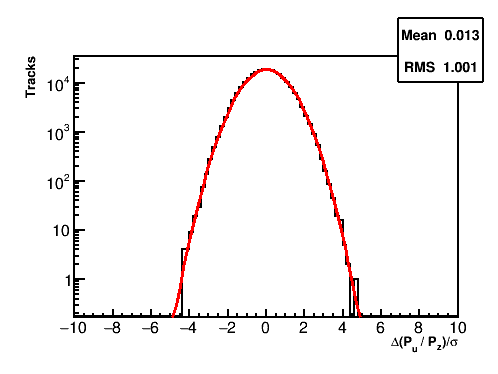
\includegraphics[width=\textwidth]{Vacuum_TruthPull_PuPz}
            \caption{$P_{u}/P_{z}$}
        \end{subfigure}
        \begin{subfigure}[t]{0.45\textwidth}
            \centering
            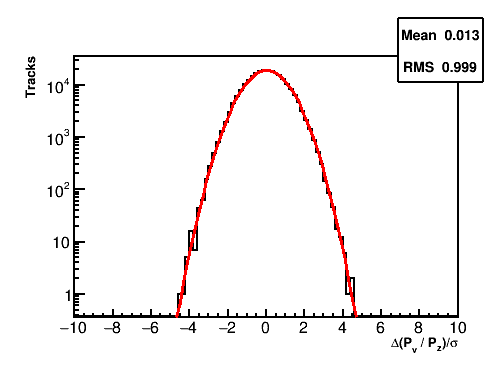
\includegraphics[width=\textwidth]{Vacuum_TruthPull_PvPz}
            \caption{$P_{v}/P_{z}$}
        \end{subfigure}%
        \vspace{2mm}
        \begin{subfigure}[t]{0.45\textwidth}
            \centering
            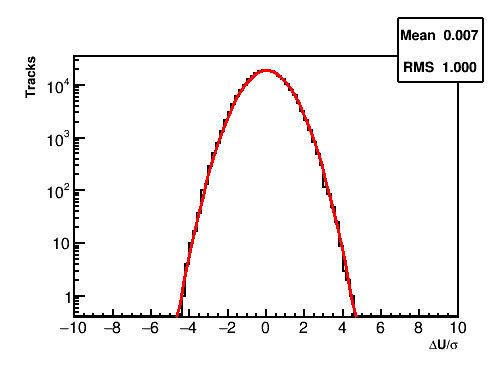
\includegraphics[width=\textwidth]{Vacuum_TruthPull_U}
            \caption{$U$}
        \end{subfigure}
        \begin{subfigure}[t]{0.45\textwidth}
            \centering
            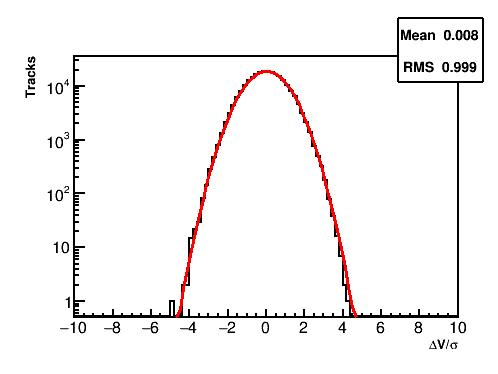
\includegraphics[width=\textwidth]{Vacuum_TruthPull_V}
            \caption{$V$}
        \end{subfigure}% 
    \caption[Track parameter truth pulls for fitted tracks in vacuum]{Truth pulls for the five fitted track parameters at the starting plane of the track, for tracks in vacuum with no material effects. The plots are shown on a log scale, and each are fit to a Gaussian in red. Each fit is consistent to a unit Gaussian with a mean of zero and an RMS of 1, showing that the track fitting is working properly. Only tracks which have failed due to Geant4 reasons are excluded.}
    \label{fig:VacuumTruthPulls}
    \end{figure}



\subsection{Material correlations}


Random processes due to material contribute to the error matrix in \equref{eq:errormatrix} as described in \secref{sub:Geane}. The random scattering of a particle trajectory at one plane means that there is an extra correlated error in all further planes, see \figref{fig:MaterialScatteringErrorDistance}. \equref{eq:chi2sum} does not take into account these material correlations between measurement planes when fitting the track. While it provides a decent approximation of the best fit track in the low material tracker, the \chisq distribution is noticeably off as shown in \figref{fig:Chi2MaterialNoCorrelations}. To calculate a better estimate of the trajectory, a more general version of the \chisq equation is used:
        \begin{align} \label{eq:chi2full}
            \chi^2 = (\vec{p}-\vec{x})^{T} (\sigma^{-1}) (\vec{p}-\vec{x})
        \end{align}
Here $\vec{x}$ and $\vec{p}$ are a $5N \times 1$ vectors of the measured and predicted track parameters respectively, where $N$ is the number of planes hit, and these objects are the combined vectors of $5 \times 1$ counterparts. Similarly, $\sigma$ is a $5N \times 5N$ matrix, where the $5 \times 5$ diagonal block matrices are the individual plane error matrices described before, calculated between plane 0 and $N$. Calculating the \chisq is now recasted from a sum over measurement planes into a single large linear algebra equation. At this point both calculations of the \chisq's are equivalent.


\begin{figure}[]
  \centering
  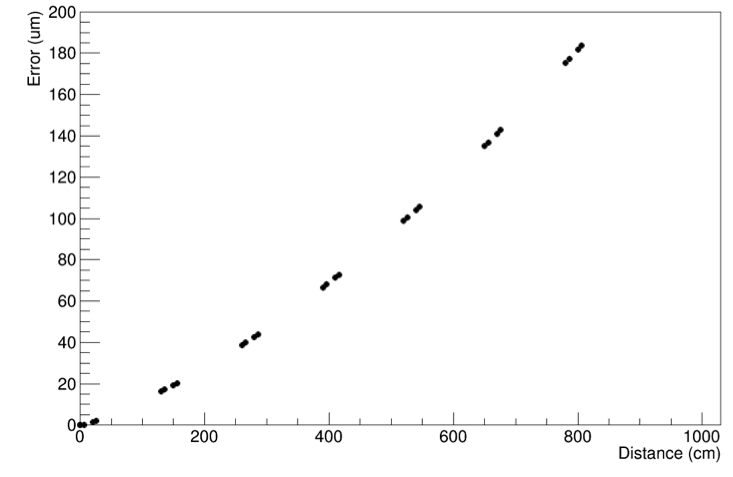
\includegraphics[width=0.6\textwidth]{MaterialScatteringErrorDistance}
    \caption[Material scattering error in tracker]{RMS error between the true track position and the average track position as a function of distance through the tracker. This error increases as a particle passes through more and more material. Each black point indicates the location of a straw measurement layer. If a track goes through the whole detector, on average the true position is nearly \mum{200} different from the average one. \textbf{careful here}}
    \label{fig:MaterialScatteringErrorDistance}
\end{figure}

\begin{figure}[]
  \centering
  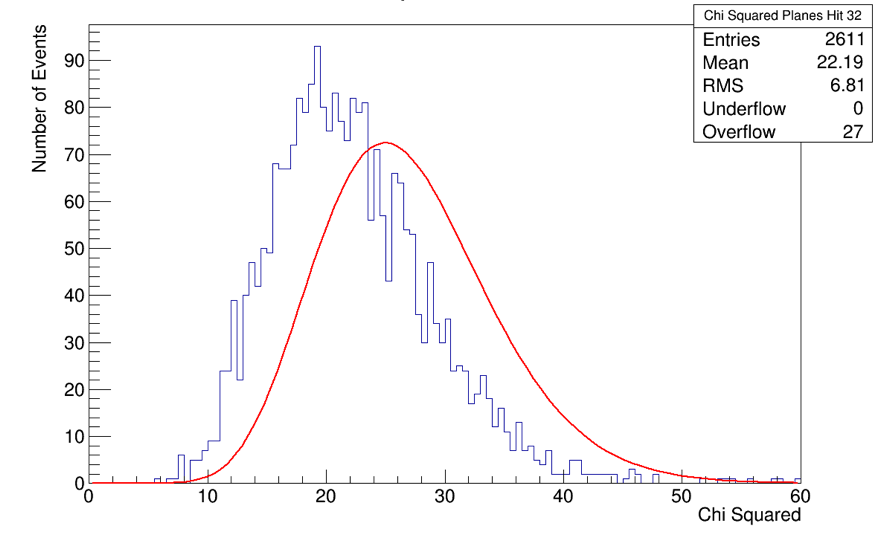
\includegraphics[width=0.6\textwidth]{Chi2MaterialNoCorrelations}
    \caption[\chisq for fitted tracks including material effects but no correlations]{The \chisq distribution for fitted tracks including material effects but excluding correlations in the calculation. The \chisq distribution is noticably different from the correct curve in red. \textbf{Axes labels and stats box don't look like previous plots, but not sure I can fix this besideds overlaying stuff.}}
    \label{fig:Chi2MaterialNoCorrelations}
\end{figure}



The new format however allows for the material correlations between planes to be included, where these correlations are added as $5 \times 5$ matrices in the off-diagonal blocks of the new large error matrix. The upper diagonals are given by 
    \begin{align} \label{eq:corr}
        \sigma_{MN} = T_{MN} \sigma_{N}, 
    \end{align}
where $\sigma_{MN}$ is the material correlation matrix between plane $M$ and plane $N$, $T_{MN}$ is the transport matrix between the two planes, and $\sigma_{N}$ is the ordinary error matrix as calculated from the 0 starting plane. \textbf{Need to cite or prove this equation, should do the latter but I can't quite remember the derivation at the moment.} The lower diagonals are just the transpose of \equref{eq:corr}. The \chisq is minimized in the same way as was done in the previous section such that the improvement to the starting track parameters $\Delta p_{0}$ remains a $5 \times 1$ vector and is given by
    \begin{align} \label{eq:deltafull}
        \Delta p_{0} &= \sigma_{p_{0}} \tau^{T}\sigma^{-1}(\vec{x}-\vec{p}), \\
        \sigma_{p_{0}} &= [\tau^{T} \sigma^{-1} \tau ]^{-1},
    \end{align}
where $\tau$ is a $5N \times 5$ object of the individual transport matrices combined together.


% Sentence from track fitting doc on calculation of correlation matrix but which I don't think makes much sense
% This follows from equation \ref{eq:errormatrix} evaluated at plane M with respect to a path length from plane N, and not plane 0, which is equivalent to \ref{eq:corr}. 


Because $\sigma$ is such a large matrix, $5N \times 5N$ where $N$ ranges from \SIrange{6}{32}{}, one can imagine that inverting it is a slow process. The tracking must have a certain amount of speed for the data to be efficiently processed and fit, which makes these inversions unfeasible. Note however that the diagonal errors of infinity values for non-measured parameters would reduce all the corresponding rows and columns to 0 after the inversion, in the same way as described before. This fact can be taken advantage of by removing said rows and columns that would contribute nothing to the \chisq anyway, and thus reducing the $5N \times 5N$ size to $N \times N$. The corresponding rows and columns of the unmeasured parameters in the combined transport matrix $\tau$ and $5N \times 1$ residual vector are also removed, resulting in an $N \times 5$ matrix for $\tau$ and an $N \times 1$ vector for the residuals. The covariance matrix $\sigma_{p_{0}}$ remains a $5 \times 5$ matrix. This improves the speed of the \chisq calculation dramatically, while leaving the final calculation unaffected\footnote{Note that these element removals are done just before the final calculation of the \chisq and fit to the track and not at the beginning of the algebra, otherwise the plane material correlations are not properly included.}. 

%Besides this $N \times N$ matrix inversion method, there is another way to do the inversion in a faster manner, which is described in \refref{trajfit}, but was not used here. % This is kind of an odd thing to say and I wouldn't know how to justify it - it would improve the track fitting speed, but most of the time is spent in the propagation phase so it doesn't matter too much in the end


\subsection{Fits to simulated tracks including material effects}

Once the material correlations are properly included, the \chisq distribution is repaired, as shown in \figref{fig:MaterialGoodnessOfFit}. The plots in this section show the results of the track fitting in the full \gmtwo Geant4 simulation with material effects turned on. Truth measurements with \mum{150} smearing are once again used as the measured hits, and a cut of $\SI{3}{\MeV}$ on the true simulated energy loss is made to remove tracks which would result in poor fits anyways. The comparison between the simulated and reconstructed energy loss for fitted tracks is shown in \figref{fig:EnergyLossComparison}. While there is a noticable difference, the energy loss in general is small so it is acceptable. Truth pulls for the tracks are shown in \figref{fig:MaterialTruthPulls}. It can be seen that there is a slight spread in results due to the material effects. This is to be expected and the vast majority of tracks still fit well. The number of iterations it takes to fit a track is shown in \figref{fig:Iterations}. The number of planes a track hits and the corresponding momentum dependence is shown in \figref{fig:NumberOfPlanesHit}. The total momentum distribution and residuals to truth are shown in \figref{fig:MaterialTotalMomentum}. The track fitting has a momentum resoltion of approximately 2\% with just a slight dependence on the momentum of the track.

After the track fitting has determined the best fit parameters in the $UV$ space, the returned parameters can be turned back into the tracker reference frame coordinates. Plots for the fitted vertical and horizontal momenta, positions, and corresponding residuals are shown in Figures~\ref{fig:MaterialFittedMomentaComponents} and \ref{fig:MaterialFittedPositionComponents}. The forward momenta plots are omitted since the majority of the total momenta is in the forward direction. More extensive plots than what is shown here can be found in \refref{trackfittingdoc}.


    \begin{figure}[]
    \centering
        \begin{subfigure}[t]{0.45\textwidth}
            \centering
            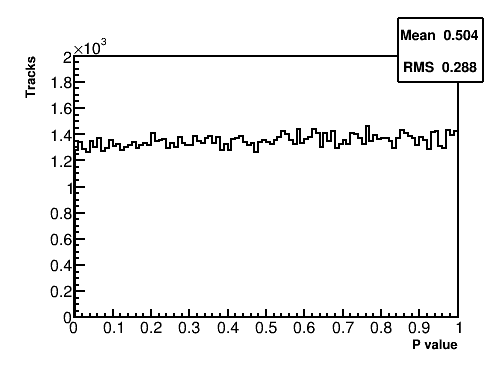
\includegraphics[width=\textwidth]{MaterialTruthLR_Pvalue}
            \caption{P value distribution for all tracks.}
        \end{subfigure}
        \begin{subfigure}[t]{0.45\textwidth}
            \centering
            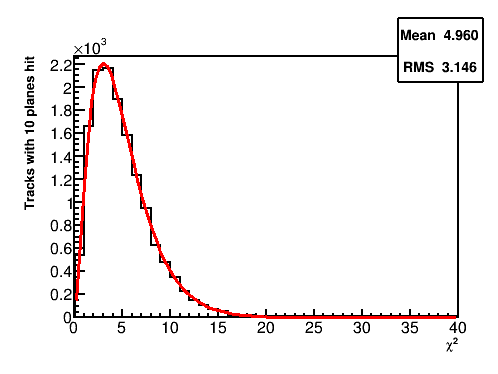
\includegraphics[width=\textwidth]{MaterialTruthLR_Chi2}
            \caption{\chisq distribution for tracks which hit 10 planes.}
        \end{subfigure}
    \caption[P value and \chisq distribution for fitted tracks in the \gmtwo Geant4 simulation with material effects included]{Goodness-of-fit distributions for fitted tracks in the full \gmtwo Geant4 simulation with material effects included. The P value distribution is flat, and the \chisq distribution matches a normalized \chisq pdf for 5 degrees of freedom which is overlayed in red.}
    \label{fig:MaterialGoodnessOfFit}
    \end{figure}

    \begin{figure}[]
      \centering
      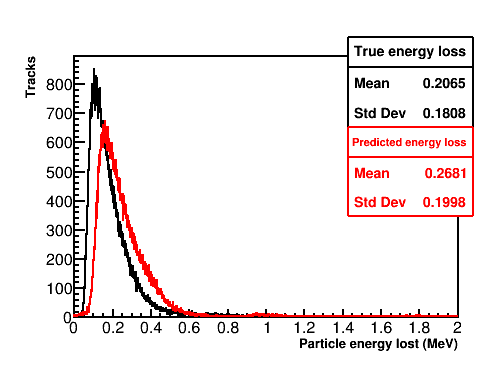
\includegraphics[width=.6\textwidth]{MaterialTruthLR_EnergyLost}
        \caption[Simulated true energy loss vs Geane predicted energy loss for tracks]{Simulated true energy loss (black) vs Geane predicted energy loss (red) for fitted tracks. As shown there is a mismatch between the two. This is acceptable as the energy loss is in general very small compared to the total momentum of each track, $200\keV \ll 2 \GeV$. Sources of energy loss come from ionization and bremsstrahlung processes, which account for the long Landau tail running off to infinity. Originally the Geane physics calculations were taking too much energy away due to bremsstrahlung processes in our low material tracker, so the energy loss calculations were modified slightly \cite{trackfittingdoc}.}
        \label{fig:EnergyLossComparison}
    \end{figure}

    \begin{figure}[]
    \centering
        \begin{subfigure}[t]{0.45\textwidth}
            \centering
            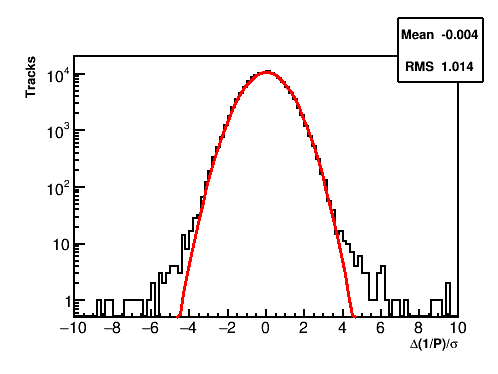
\includegraphics[width=\textwidth]{MaterialTruthLR_TruthPull_1P}
            \caption{$1/P$}
        \end{subfigure}%

        \vspace{2mm}
        \begin{subfigure}[t]{0.45\textwidth}
            \centering
            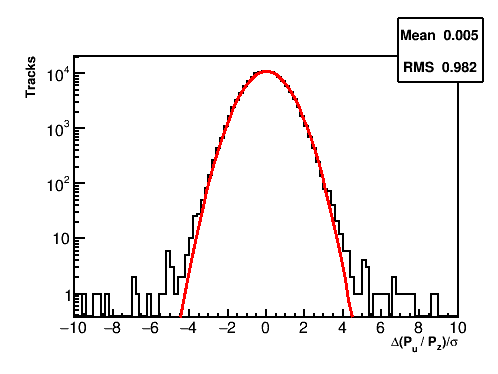
\includegraphics[width=\textwidth]{MaterialTruthLR_TruthPull_PuPz}
            \caption{$P_{u}/P_{z}$}
        \end{subfigure}
        \begin{subfigure}[t]{0.45\textwidth}
            \centering
            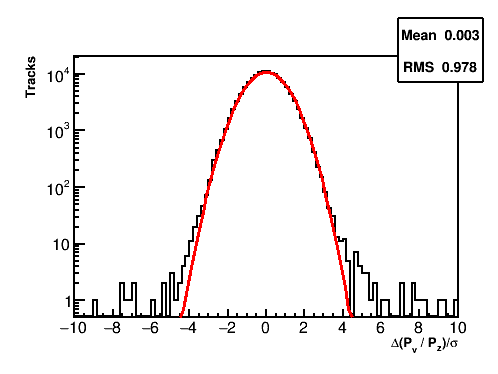
\includegraphics[width=\textwidth]{MaterialTruthLR_TruthPull_PvPz}
            \caption{$P_{v}/P_{z}$}
        \end{subfigure}%
        \vspace{2mm}
        \begin{subfigure}[t]{0.45\textwidth}
            \centering
            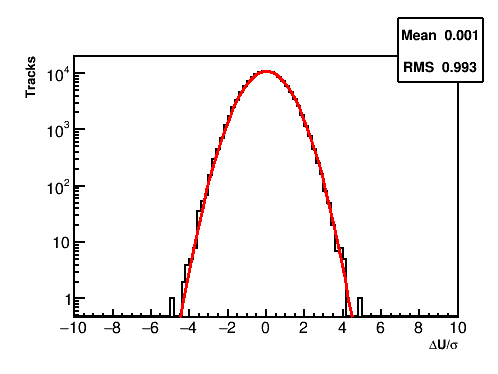
\includegraphics[width=\textwidth]{MaterialTruthLR_TruthPull_U}
            \caption{$U$}
        \end{subfigure}
        \begin{subfigure}[t]{0.45\textwidth}
            \centering
            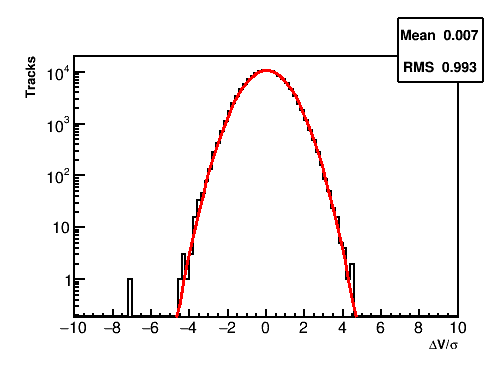
\includegraphics[width=\textwidth]{MaterialTruthLR_TruthPull_V}
            \caption{$V$}
        \end{subfigure}% 
    \caption[Track parameter truth pulls for fitted tracks in the \gmtwo Geant4 simulation with material effects included]{Truth pulls for the five fitted track parameters at the starting plane of the track for fitted tracks in the full \gmtwo Geant4 simulation with material effects included. The plots are shown on a log scale, and each are fit to a Gaussian in red. Each fit is close to a unit Gaussian with a mean of zero and an RMS of 1, but there are tracks which lie outside the Gaussian due to material effects and imperfect resulting fits.}
    \label{fig:MaterialTruthPulls}
    \end{figure}

    \begin{figure}[]
      \centering
      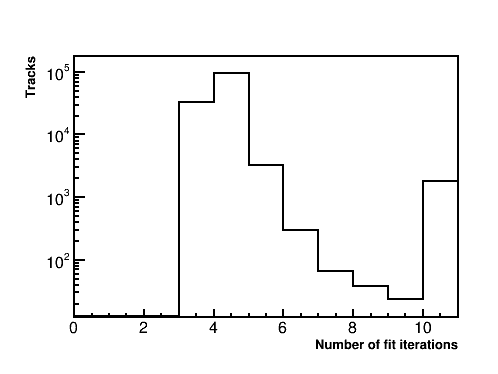
\includegraphics[width=.6\textwidth]{MaterialTruthLR_NumberIterations}
        \caption[Number of iterations for the track fitting to converge]{Number of iterations for the track fitting to converge per track. The track fitting does not take less than three iterations, and the number of iterations is capped at ten.}
        \label{fig:Iterations}
    \end{figure}


    \begin{figure}[]
    \centering
        \begin{subfigure}[t]{0.45\textwidth}
            \centering
            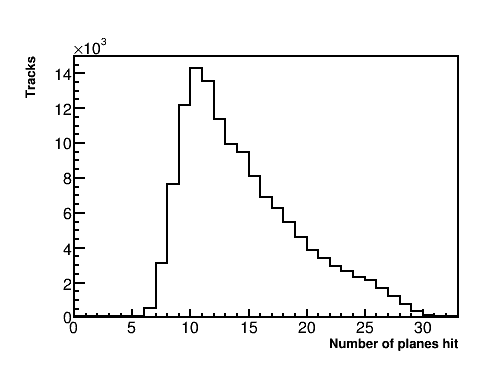
\includegraphics[width=\textwidth]{MaterialTruthLR_NumberPlanesHit}
            \caption{The number of planes hit peaks at 10, and falls off to the maximum number of planes at 32.}
        \end{subfigure}
        \hspace{5mm}
        \begin{subfigure}[t]{0.45\textwidth}
            \centering
            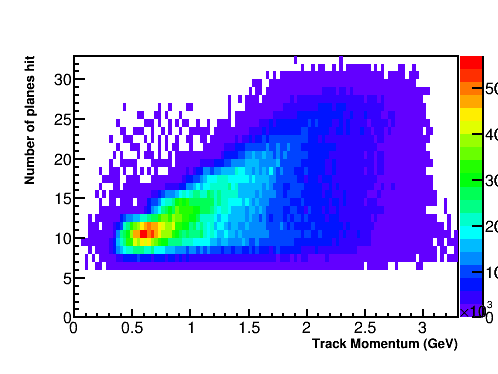
\includegraphics[width=\textwidth]{MaterialTruthLR_NumberPlanesHitVsP}
            \caption{The number of planes hit vs the momentum of the track. Tracks with higher momentum in general hit more planes.}
        \end{subfigure}
    \caption[Number of planes hit for fitted tracks]{Number of planes hit per track (left) and the momentum dependence (right).}
    \label{fig:NumberOfPlanesHit}
    \end{figure}


    \begin{figure}[]
    \centering
        \begin{subfigure}[t]{0.6\textwidth}
            \centering
            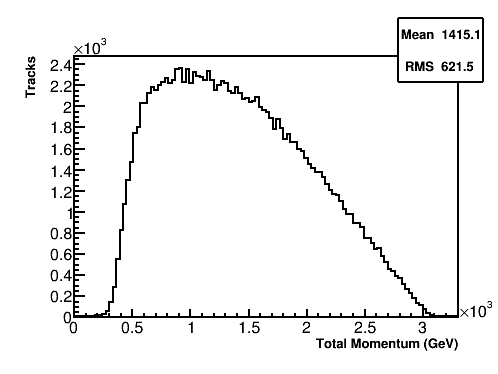
\includegraphics[width=\textwidth]{MaterialTruthLR_Fitted_PTotal}
            \caption{The fitted momentum distribution for tracks which tails off at approximately the magic momentum of $\SI{3.094}{\GeV}.$}
        \end{subfigure}%

        \vspace{2mm}
        \begin{subfigure}[t]{0.45\textwidth}
            \centering
            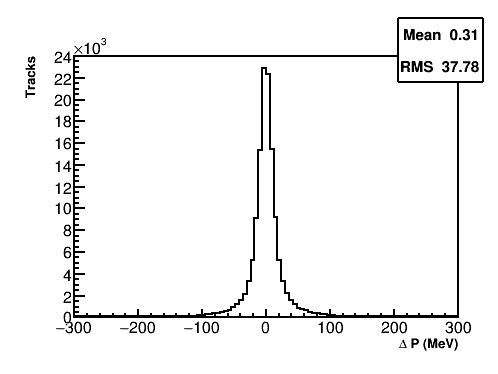
\includegraphics[width=\textwidth]{MaterialTruthLR_Fitted_PTotal_AbsResidual}
            \caption{The residual between the reconstructed and true total momentum. The RMS is approximately $\SI{40}{\MeV}$, though there are some tails which spread out from the distribution.}
        \end{subfigure}
        \hspace{5mm}
        \begin{subfigure}[t]{0.45\textwidth}
            \centering
            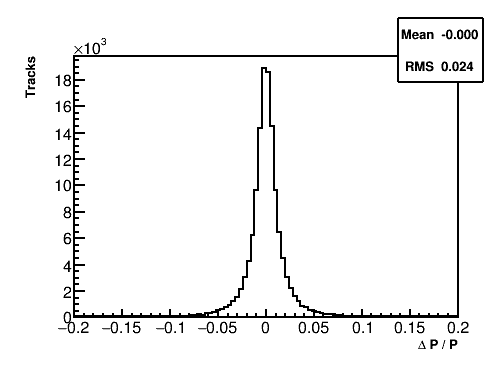
\includegraphics[width=\textwidth]{MaterialTruthLR_Fitted_PTotal_RelResidual}
            \caption{The relative residual between the reconstructed and true total momentum. The RMS is approximately $\SI{2.4}{\%}$. This plot includes tracks of all momenta; in general the resolution of the total momentum is around 2\% for all energies.}
        \end{subfigure}%
    \caption[Fitted track momentum distribution and corresponding residuals to truth]{Fitted track momentum distribution and corresponding residuals to truth.}
    \label{fig:MaterialTotalMomentum}
    \end{figure}


    \begin{figure}[]
    \centering
        \begin{subfigure}[t]{0.45\textwidth}
            \centering
            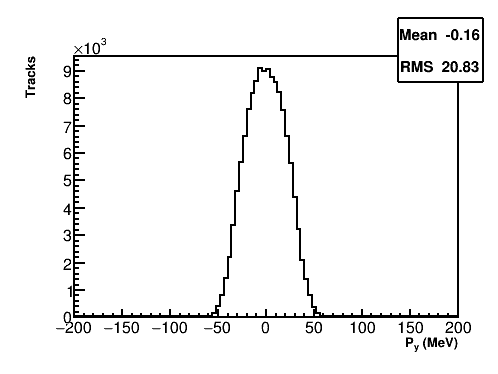
\includegraphics[width=\textwidth]{MaterialTruthLR_Fitted_Py}
            \caption{Vertical momentum distribution. This distribution is bounded by the storage region which limits the vertical momentum of the muons and by extension the decay positrons.}
        \end{subfigure}
        \hspace{5mm}
        \begin{subfigure}[t]{0.45\textwidth}
            \centering
            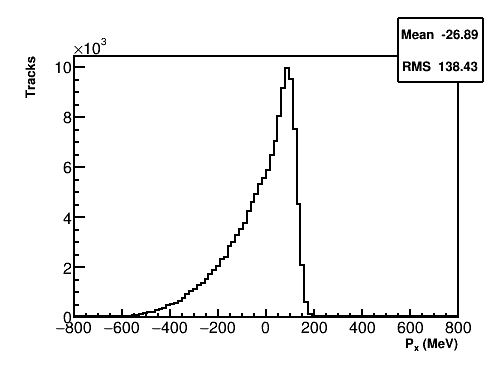
\includegraphics[width=\textwidth]{MaterialTruthLR_Fitted_Px}
            \caption{Horizontal momentum distribution. This distribution has an interesting shape due to the acceptance of the tracker. It is perhaps more informative to look at the radial momentum distribution, which is shown in \figref{fig:TracksDataMCSecond}.}
        \end{subfigure}
        \vspace{2mm}
        \begin{subfigure}[t]{0.45\textwidth}
            \centering
            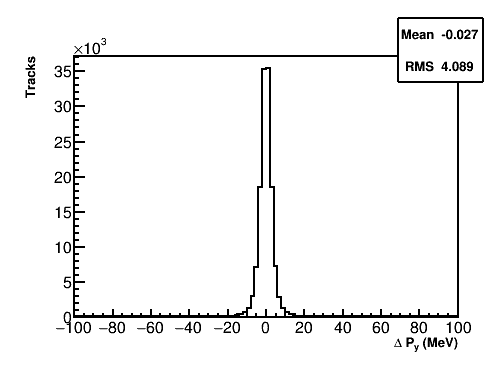
\includegraphics[width=\textwidth]{MaterialTruthLR_Fitted_Py_AbsResidual}
            \caption{The vertical momentum residual, which has a width of about $\SI{4}{\MeV}$.}
        \end{subfigure}%
        \hspace{5mm}
        \begin{subfigure}[t]{0.45\textwidth}
            \centering
            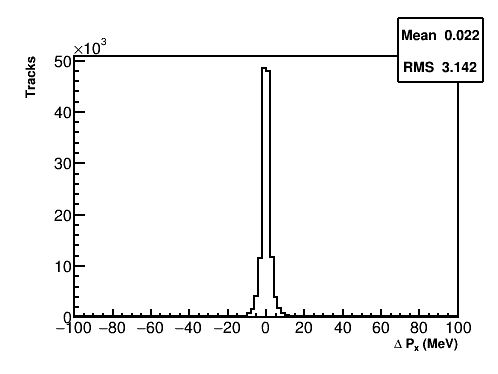
\includegraphics[width=\textwidth]{MaterialTruthLR_Fitted_Px_AbsResidual}
            \caption{The horizontal momentum residual, which has a width of about $\SI{3}{\MeV}$.}
        \end{subfigure}%
    \caption[Fitted track vertical and horizontal momenta and corresponding residuals to truth]{Shown are the fitted vertical and horizontal momentum components (top) for tracks at the entrance to the tracker, and their residuals to truth (bottom).}
    \label{fig:MaterialFittedMomentaComponents}
    \end{figure}

    \begin{figure}[]
    \centering
        \begin{subfigure}[t]{0.45\textwidth}
            \centering
            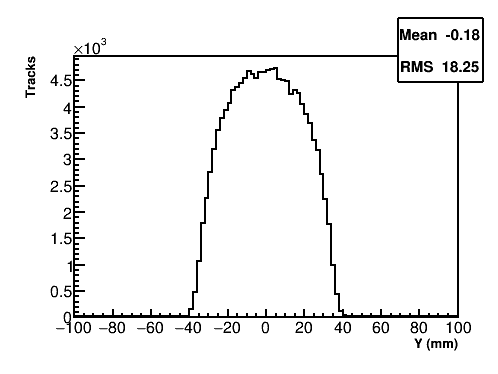
\includegraphics[width=\textwidth]{MaterialTruthLR_Fitted_Y}
            \caption{Vertical position distribution. This distribution is bounded by the storage region which limits the vertical positions of the muons and by extension the decay positrons.}
        \end{subfigure}
        \hspace{5mm}
        \begin{subfigure}[t]{0.45\textwidth}
            \centering
            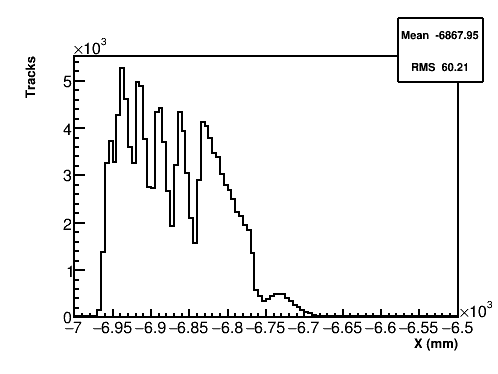
\includegraphics[width=\textwidth]{MaterialTruthLR_Fitted_X}
            \caption{Horizontal position distribution. This distribution has an interesting shape due to the acceptance of the tracker. It is perhaps more informative to look at the radial position distribution, which is shown later in \figref{fig:TracksDataMCSecond}.}
        \end{subfigure}
        \vspace{2mm}
        \begin{subfigure}[t]{0.45\textwidth}
            \centering
            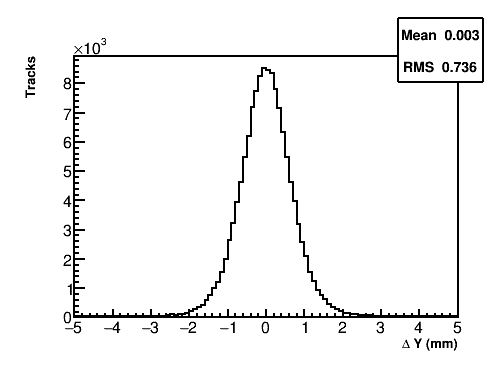
\includegraphics[width=\textwidth]{MaterialTruthLR_Fitted_Y_AbsResidual}
            \caption{The vertical position residual, which has a width of about \mum{740} at the entrance of the tracker. This is expected from geometry arguments with the angles of the straws which measure mostly horizontally.}
        \end{subfigure}%
        \hspace{5mm}
        \begin{subfigure}[t]{0.45\textwidth}
            \centering
            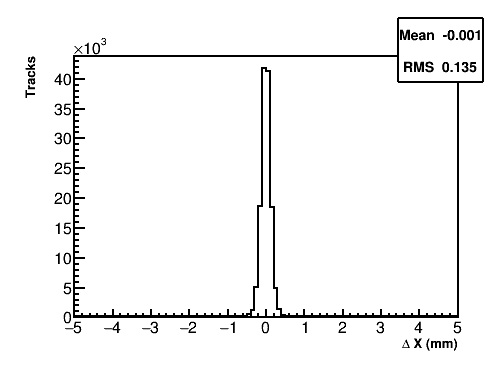
\includegraphics[width=\textwidth]{MaterialTruthLR_Fitted_X_AbsResidual}
            \caption{The horizontal position residual, which has a width of about \mum{140} at the entrance of the tracker. This is close to the input straw resolution of \mum{150} but slightly better due to the face that both straws measure mostly horizontally.}
        \end{subfigure}%
    \caption[Fitted track vertical and horizontal positions and corresponding residuals to truth]{Shown are the fitted vertical and horizontal position components (top) for tracks at the entrance to the tracker, and their residuals to truth (bottom).}
    \label{fig:MaterialFittedPositionComponents}
    \end{figure}


\clearpage % do this so left-right section isn't separated by 5 pages of plots - might want to remove this down the line depending on how my edits change the text


\subsection{Left right ambiguity and fit modes}
\label{sub:leftright}


Before actual data can be fitted, the left-right ambiguity problem needs to be dealt with. Since straws only measure drift circles and not actual U or V positions, and since tracks are in general passing forwards through the detector, there is an ambiguity as to which side of the wire a particle passed for each hit. In general if even a single left-right choice for a hit is wrong then a track will fit poorly. There are a couple of different track fitting modes used to deal with this problem, which are detailed in \refref{trackfittingdoc} and summarized here and in \refref{leftrightpresentation}.

\subsection*{\texttt{wireFit}}

The first fit to any set of tracks in data is to do a fit to the wire centers, which requires no left-right information. The errors on the measured hits are set as the RMS of a uniform distribution with a width of a straw diameter. After a wire fit, an approximation of the best fit track is acquired which provides some left-right information. The number of fitting iterations is capped at three for the wire fit.

\subsection*{\texttt{mainfit}}

The primary fit mode for analyzing data is called \texttt{mainFit}. After the wire fit is completed, the predicted track parameters at each measurement plane are compared with the locations of the wires for the straws that were hit. The left-right choices for each hit are set depending on which side of the wire the predicted track passed. The measured hit positions and errors are updated from the wire values to the angular-corrected DCA values based on the the left-right choices of each hit, and the fitting is repeated. At each iteration of the fitting, the left-right choices for each hit are updated based on where the previous predicted track parameters ended up. This is the fastest fit mode and with this method about 66\% of tracks are fit well. Since there is no shortage when it comes to statistics for positron tracks, this is acceptable.


\subsection*{\texttt{fullSeqFit}}

The secondary fit mode is called \texttt{fullSeqFit}. This fit mode does a better job of determining the left-right choices for the hits in a track, but is much slower than \texttt{mainFit}. Since there is no statistics problem when it comes to tracks, this fit mode is usually ignored. Here is given a short summary, see \refref{trackfittingdoc} for more technical details on all parts of this fitting mode.

After a wire fit, the geometry of the straw layers is used to resolve some of the left-right choices for a hit on a track. The left-right ambiguity is partially resolved through the shift in layers for each view as detailed in \secref{sec:StrawTrackers}, where if a particle passes straight through both layers in a view it can be seen to go to the left of one wire and the right of the other. This implies that for curved tracks with certain angles through tracker modules, the left-right choices for some hits are known precisely \cite{JoeLR}. For these hit planes the left-right choices are locked in and taken as known for the rest of the fitting.

For the remaining hits where the left-right choices are unknown, an approximate \chisq is calculated for each combination of left-right choices, $2^{N_{\text{unknown}}}$. This \chisq is calculated using the same formula as in the full fitting 
with the measured parameters set to the different left-right combinations, \equref{eq:chi2full}, but using the Geane transport and error matrices calculated by the wire fit instead of from a fit to the left-right choice measured parameters. Calculating this \chisq for each combination is slow, so this process is sped up by only checking the left-right combinations for the U or V hit layers at a time respectively, $2^{N_{\text{U,unknown}}} + 2^{N_{\text{V,unknown}}} \ll 2^{N_{\text{unknown}}}$. This \chisq calculation allows for a measure of how good a left-right combination is to be determined without having to propagate every track in Geane for the full fitting. The tracks with the best combinations and smallest approximate \chisq's are then fitted with the full Geane propagation and \chisq minimization algorithm. Typically the best 10 to 15 combinations are fitted, and the final track with the best \chisq is taken as the true track. This gets the left-right choices for the fitted track right 99\% of the time with simulated data, but is very slow due to the combination checking and the Geane propagation for each of the best track left-right combinations. If the track fitting can be sped up significantly or a majority of the left-right choices constrained upstream somehow, then this fit mode would be more useful. 




\subsection{Fits to tracks from data and comparison with Monte-Carlo}


Fits to data are done with \texttt{mainFit}. Due to imperfect left-right assignments and the use of real DCA and DCA error measurements, the tracks from data are naturally more messy. See \figref{fig:pValueData} for a plot of the goodness-of-fit for the tracks. While not all tracks are fitted perfectly, enough of them are fit well in order to pass on the results to the extrapolation stage. Fitted tracks to Run 1 data are compared to results from Monte-Carlo. Track times and fitted total momenta are shown in \figref{fig:TracksDataMCFirst}. Fitted track radial and vertical momentum and position distributions are shown in \figref{fig:TracksDataMCSecond}. In general the results are very similar between the two. There are mismatches in the distributions because the idealized simulation did not reflect the real run conditions at the time of this track fitting analysis. As described in \secref{sec:Run1} and explored later in \secref{sec:MuonBeamMeasurements}, the muon beam was imperfectly stored in the ring leading to the measured distributions here.


    \begin{figure}[]
        \centering
        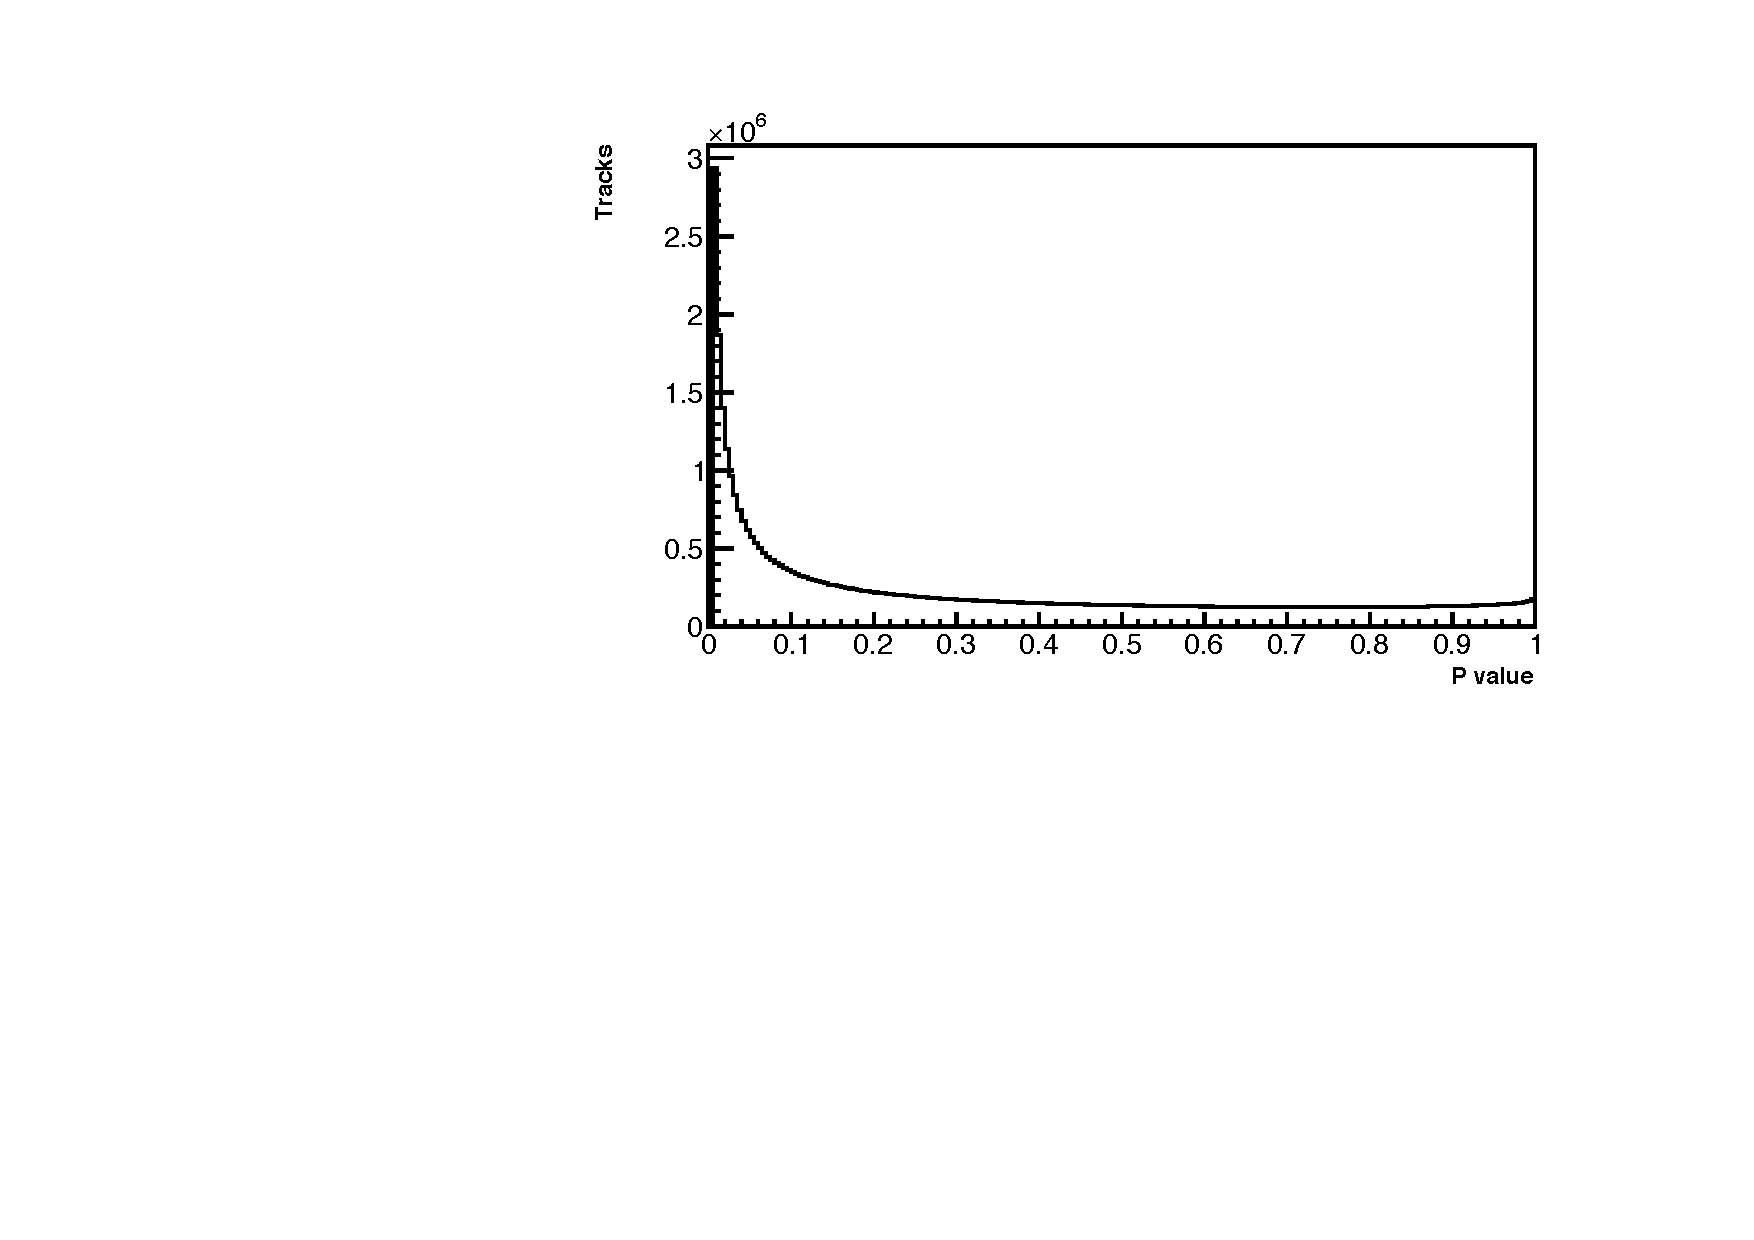
\includegraphics[width=.6\textwidth]{LatestData_Pvalue_lessCut}
        \caption[P value distribution for fitted tracks in data]{P value distribution for fitted tracks in data. A cut has been made at 1\% to remove tracks which have entirely failed the fitting. The distribution can be seen to rise towards zero where tracks have been fit but imperfectly.}
        \label{fig:pValueData}
    \end{figure}


    \begin{figure}[]
    \centering
        \begin{subfigure}[t]{0.47\textwidth}
            \centering
            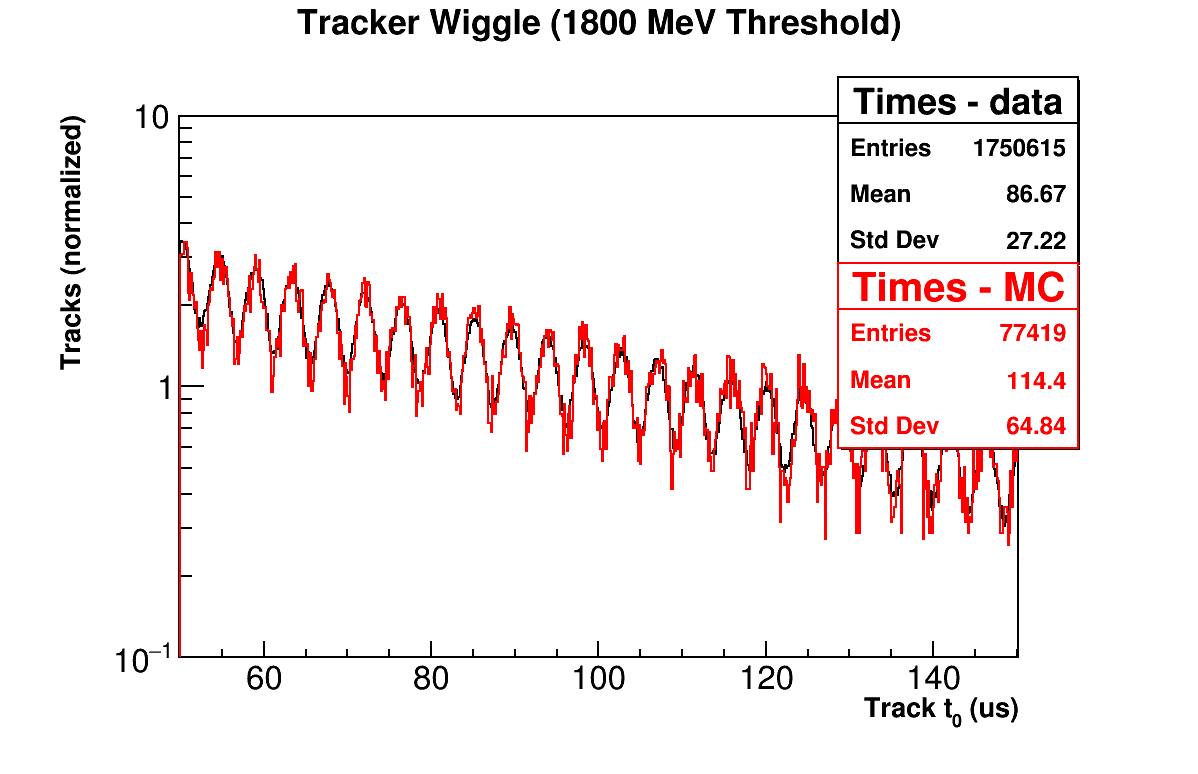
\includegraphics[width=\textwidth]{TrackerWiggleDataMC}
            \caption{Track times for tracks with energy greater than $\SI{1.8}{\GeV}$. The \gmtwo frequency can be seen in both the data and simulation.}
        \end{subfigure}
        \hspace{5mm}
        \begin{subfigure}[t]{0.47\textwidth}
            \centering
            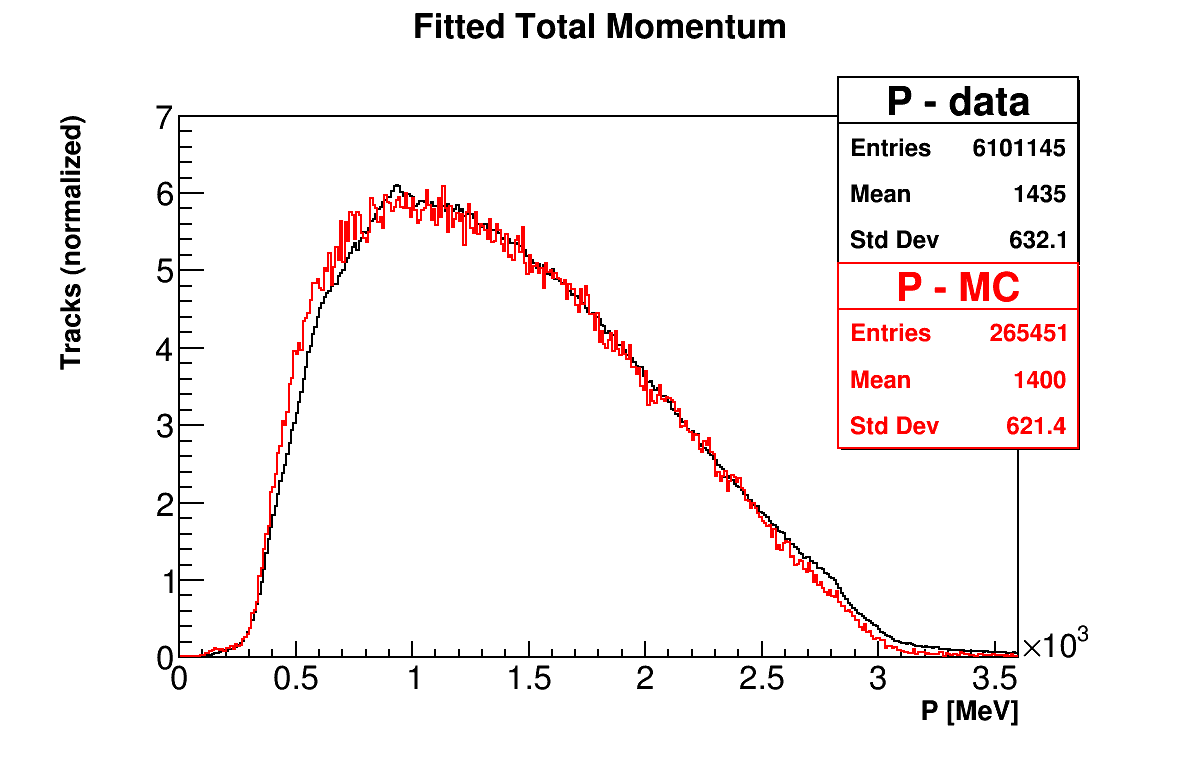
\includegraphics[width=\textwidth]{TotalMomentumDataMC}
            \caption{Fitted track total momentum, there is a very slight mismatch between data and Monte-Carlo.}
        \end{subfigure}
    \caption[Fitted tracks in data compared to Monte-Carlo, track times and total momentum]{Fitted track results in data (black) vs Monte-Carlo (red). The amount of entries in each are normalized to each other so that they can be compared. Shape differences between the two are due to a mismatch between simulation conditions and the real experiment, and not any problem with the track fitting.}
    \label{fig:TracksDataMCFirst}
    \end{figure}


    \begin{figure}[]
    \centering
        \begin{subfigure}[t]{0.47\textwidth}
            \centering
            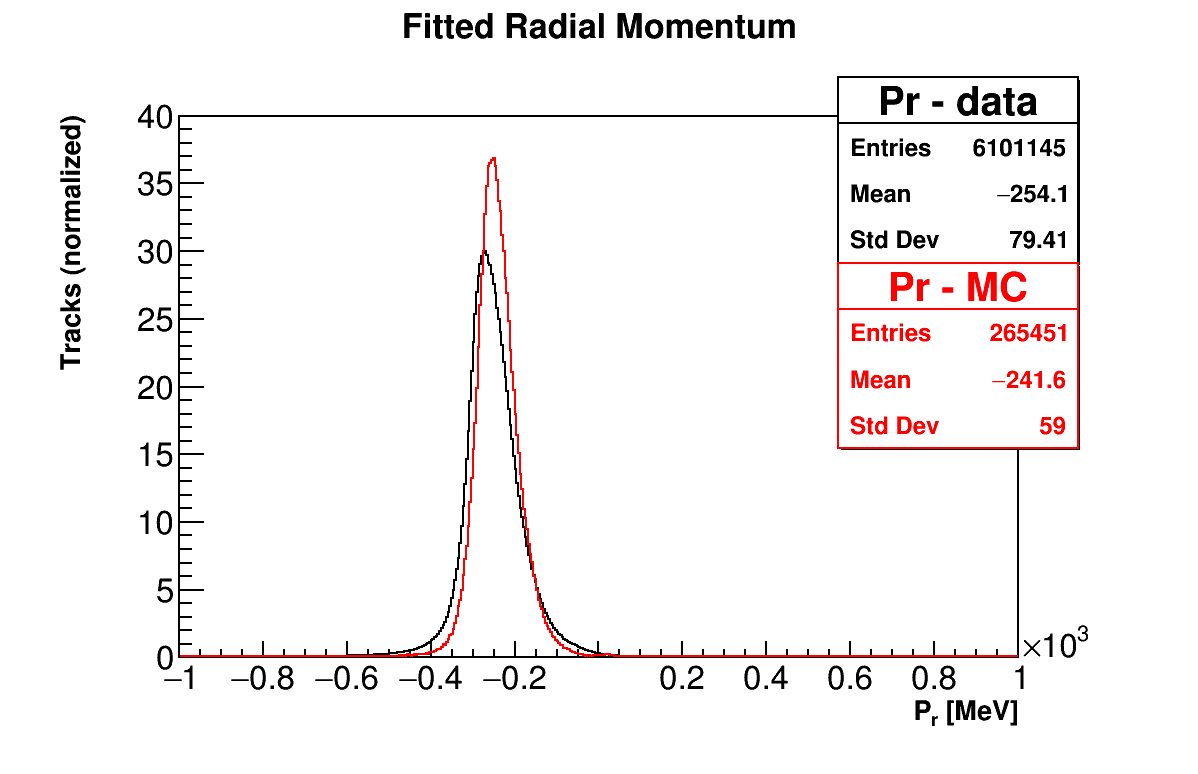
\includegraphics[width=\textwidth]{RadialMomentumDataMC}
            \caption{Fitted track radial momenta. The radial momentum of the tracks are negative as particles are curving inwards through the tracker. There is a very noticeable difference between data and Monte-Carlo results.}
        \end{subfigure}
        \hspace{5mm}
        \begin{subfigure}[t]{0.47\textwidth}
            \centering
            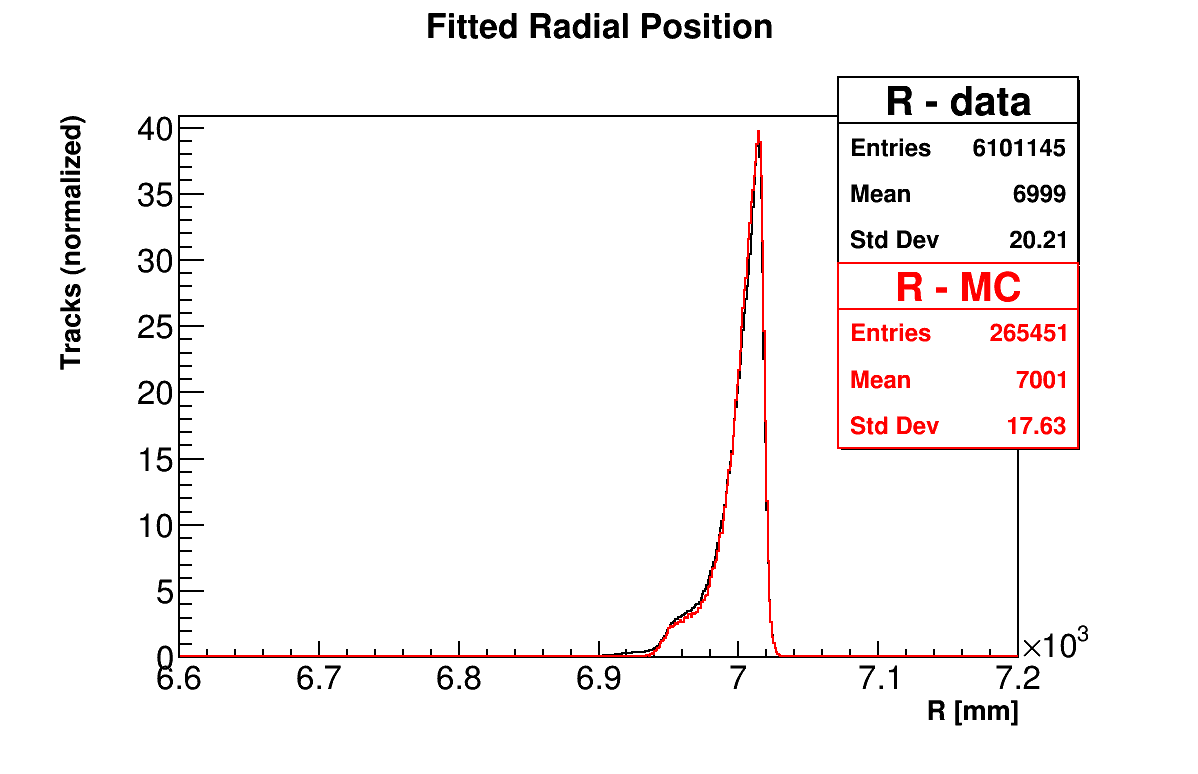
\includegraphics[width=\textwidth]{RadialPositionDataMC}
            \caption{Fitted track radial positions. The shape depends on the acceptance of the tracker and in general lies below the magic radius of $\SI{7.112}{m}$. Data and Monte-Carlo results match well.}
        \end{subfigure}
        \vspace{2mm}
        \begin{subfigure}[t]{0.47\textwidth}
            \centering
            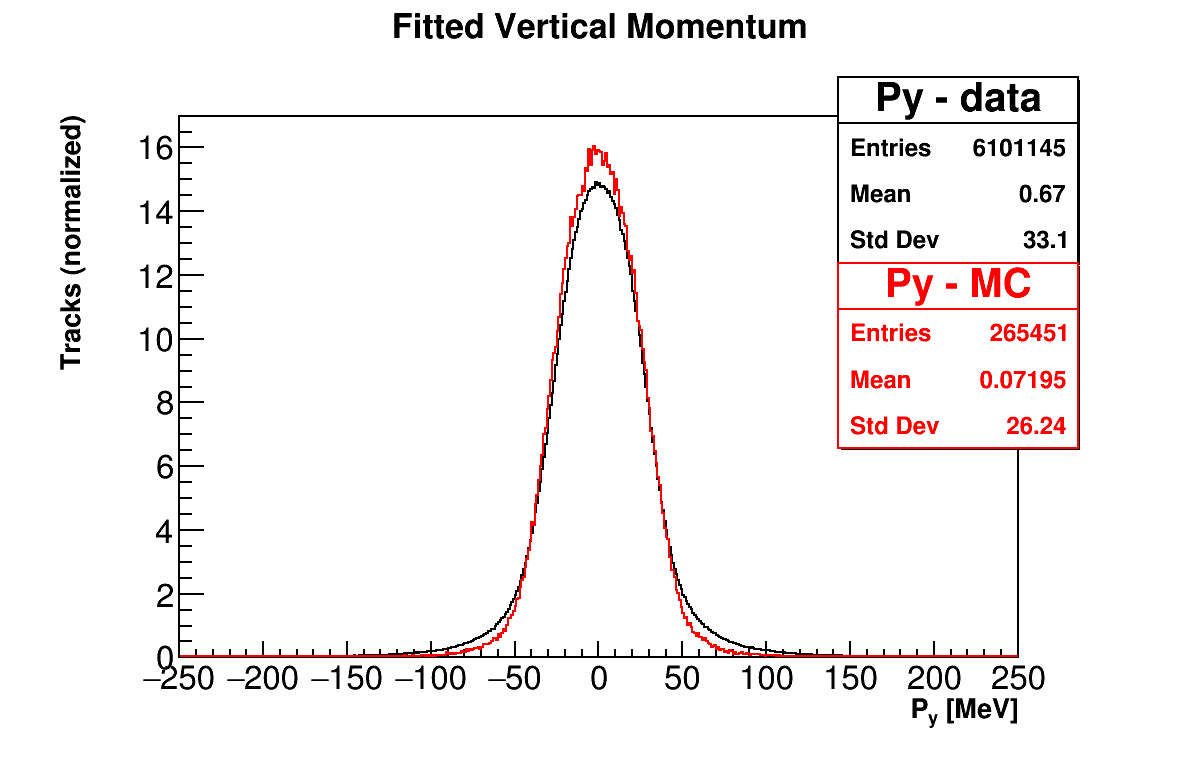
\includegraphics[width=\textwidth]{VerticalMomentumDataMC}
            \caption{Fitted track vertical momenta. The momentum is bounded by the storage region, and data has a slightly wider width than Monte-Carlo.}
        \end{subfigure}%
        \hspace{5mm}
        \begin{subfigure}[t]{0.47\textwidth}
            \centering
            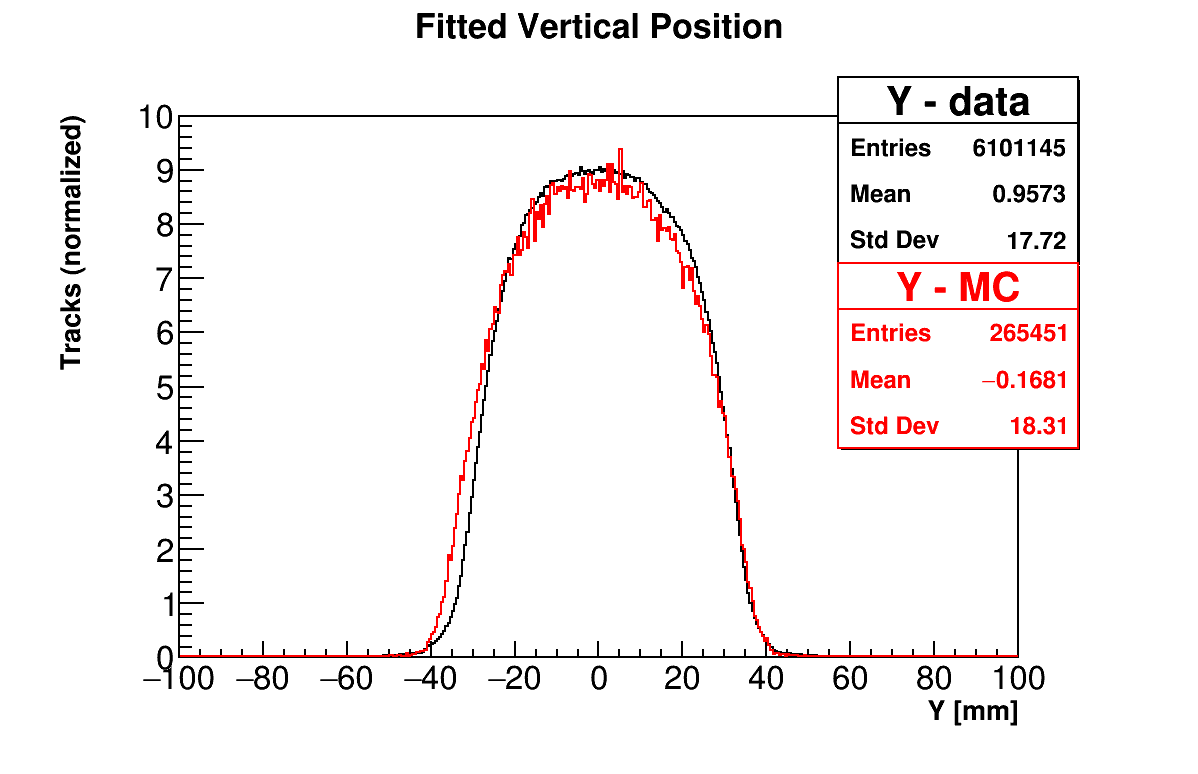
\includegraphics[width=\textwidth]{VerticalPositionDataMC}
            \caption{Fitted track vertical positions. The positions are bounded by the storage region. There is a noticeable difference between data and Monte-Carlo.}
        \end{subfigure}%
    \caption[Fitted tracks in data compared to Monte-Carlo, radial and vertical momentum and position distributions]{Fitted track results in data (black) vs Monte-Carlo (red). The amount of entries in each are normalized to each other so that they can be compared. Shape differences between the two are due to a mismatch between simulation conditions and the real experiment, and not any problem with the track fitting.}
    \label{fig:TracksDataMCSecond}
    \end{figure}



\clearpage % stopper for where I'm at 


% \subsection{In the code}

% \begin{figure}[]
%   \centering
%   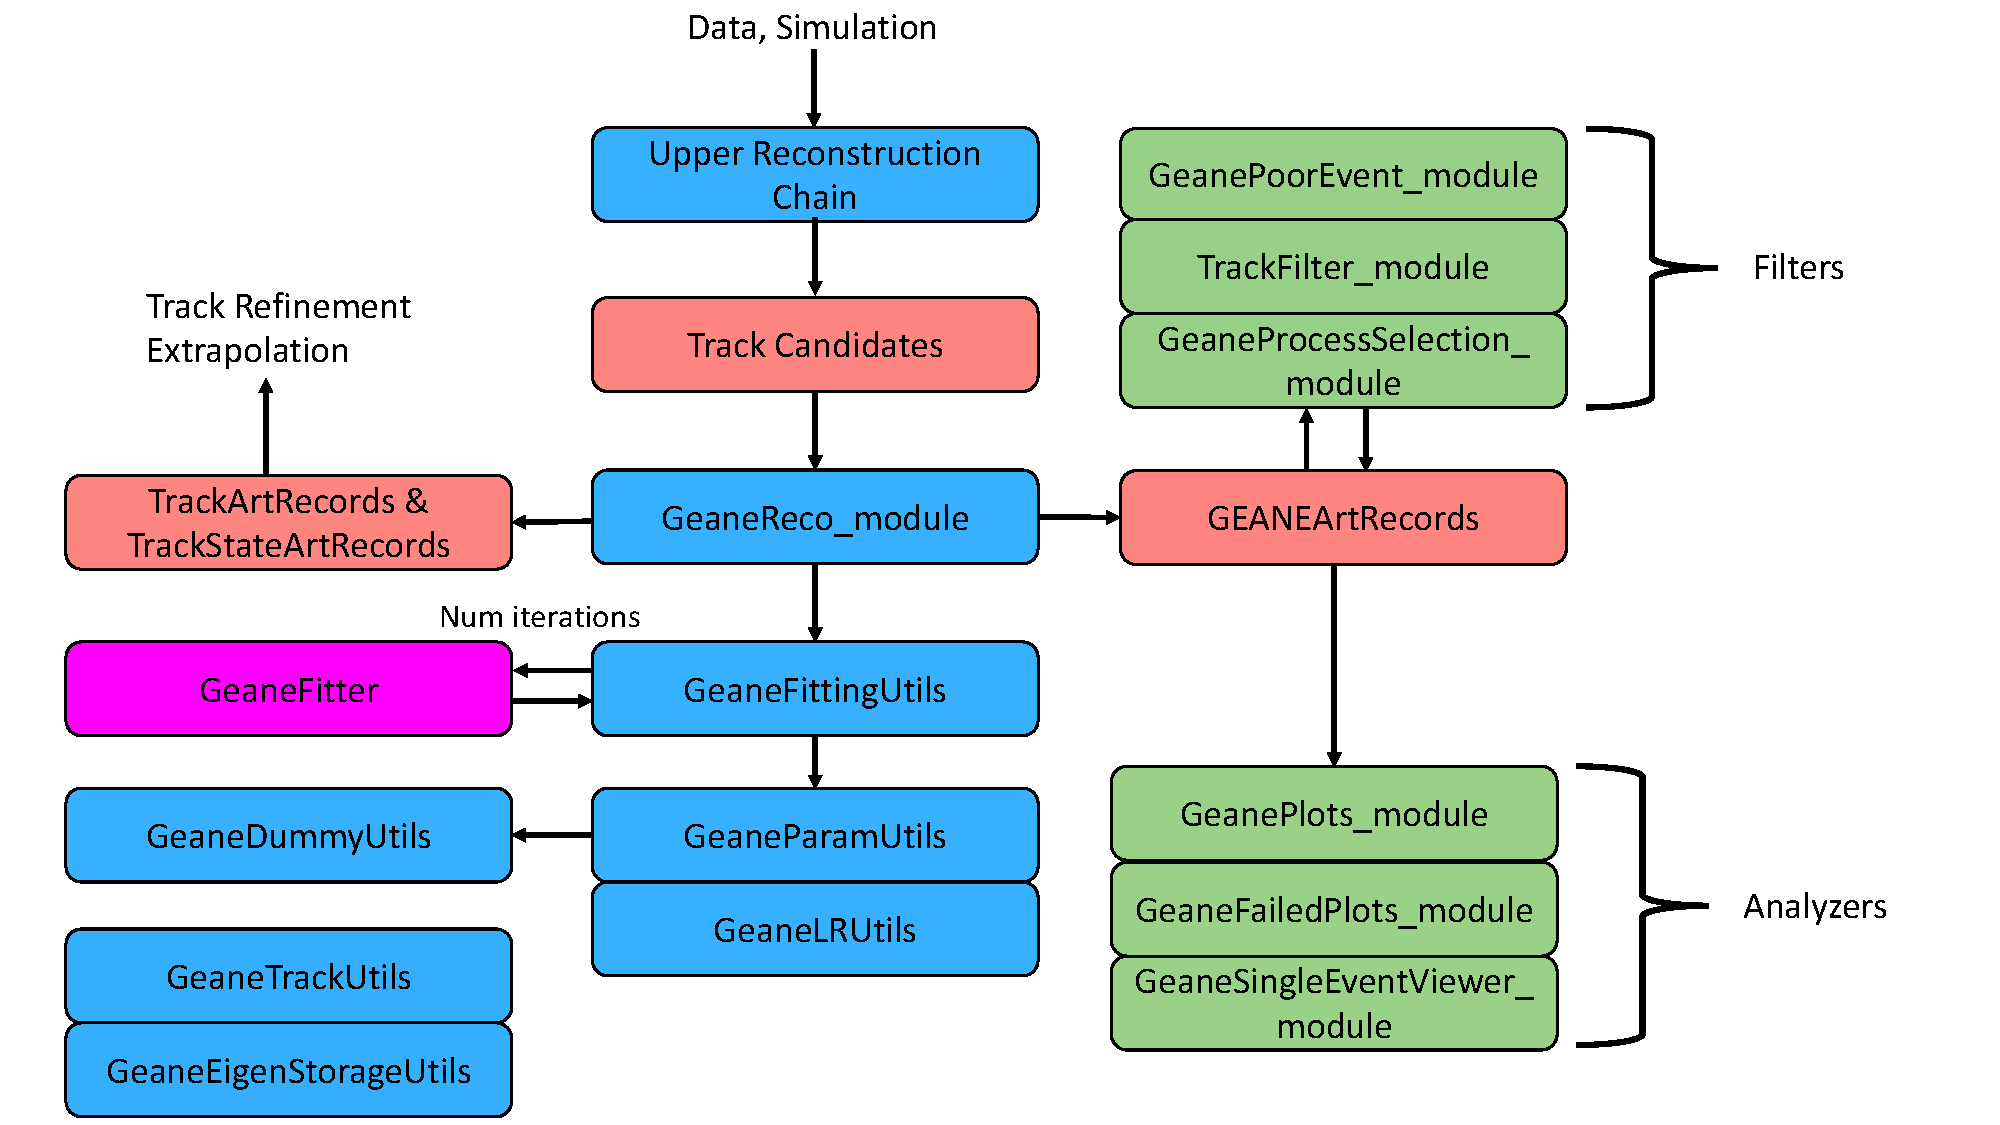
\includegraphics[width=\textwidth]{NewGeaneFlow}
%     \caption[Geane code flow]{}
%     \label{fig:NewGeaneFlow}
% \end{figure}



\section{Track extrapolation}
\label{sec:TrackExtrapolation}

The last stage of the track reconstruction is the track extrapolation. The extrapolation takes the fitted track results and either extrapolates them back to the storage region to the approximate position of the muon decay point, or forwards to the face of the calorimeter sitting right behind the tracker. The extrapolation stage utilizes a fourth order Runge-Kutta Nystr\"{o}m algorithm \cite{SCThesis} which discretely steps a trajectory through the magnetic field in the full \gmtwo Geant4 simulation, similar in some respects to the track fitting stage. At each step of the extrapolation, the updated track position and covariance matrix are compared to physical volumes in the simulation to flag tracks which have been reconstructed as likely originating from outside the storage region \cite{SCThesis,extrapolationerrors}. Because there is no fixed interaction point in the storage region, tracks are extrapolated backwards to the point of tangency where the radial momentum is equal to zero. Studies were done to verify that this approximation for the muon decay point was sufficient using truth Monte-Carlo, and it was found that a simple $\SI{1.1}{mm}$ correction to the radial decay position could be applied regardless of the momentum of the track \cite{SCThesis}. The vertical extrapolated distribution was found to have no biases. (What about the azimuthal point? Mentioned a little bit in DocDB 8564 but do I really want to go into it?) A birds eye view for tracks extrapolated back into the storage ring is shown in \figref{fig:VertexPlanView}.


\begin{figure}[]
    \centering
    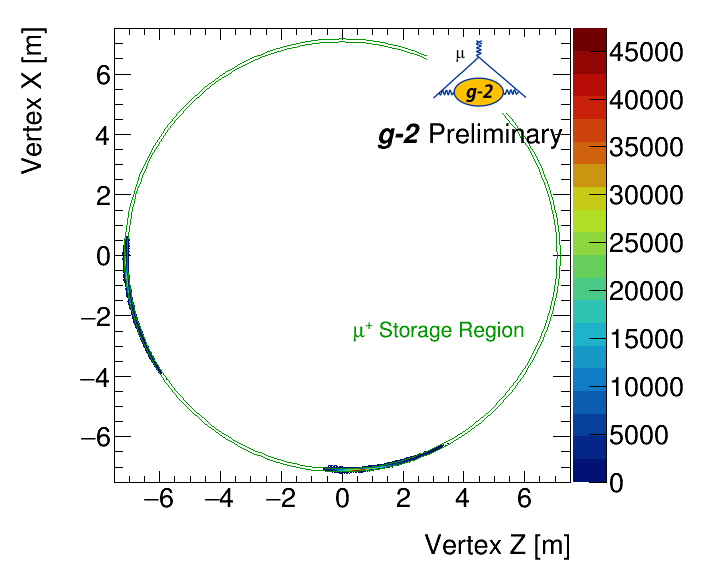
\includegraphics[width=\textwidth]{VertexPlanView}
    \caption[Birds eye view of extrapolation in ring]{A birds eye view of the extrapolation results in the storage ring. The two distributions of extrapolated tracks can be seen at the left and bottom of the figure, where the tracker sits at the heads of the distributions. It can be seen that some tracks are extrapolated multiple meters back through the storage region. (Mention anything about the cuts in this plot?)}    
    \label{fig:VertexPlanView}
\end{figure}



\section{Muon beam measurements}
\label{sec:MuonBeamMeasurements}

All stages of the track reconstruction have ultimately lead to the goal of determining muon beam parameters and dynamics. 





\begin{itemize}
    \item{Non-failed track or vertex}
    \item{No volumes hit}
    \item{Number of tracking planes hit $\geq 12$}
    \item{p value $> 5\%$}
    \item{Vertical extrapolation uncertainty: $0.5 < \sigma_{y} < \SI{3.5}{mm}$}
    \item{Radial extrapolation uncertainty: $0.5 < \sigma_{r} < \SI{5}{mm}$}
    \item{Horizontal entrance into tracker: $60 < X < \SI{150}{mm}$}
    \item{Vertical entrance into tracker: $-40 < Y < \SI{40}{mm}$}
    \item{Drift time: $0 < t_{d} < \SI{70}{ns}$}
    \item{Track UV residuals $< \mum{500}$}
    \item{Fraction of missed planes $< 30\%$}
    \item{$|$Number of U hits - number of V hits$|$ $\leq 4$}
\end{itemize}


\cite{trackcuts1,trackcuts2}




 A radial slice of the extrapolated beam distribution is shown in \figref{fig:BeamCrossSection}.

\begin{figure}[]
  \centering
  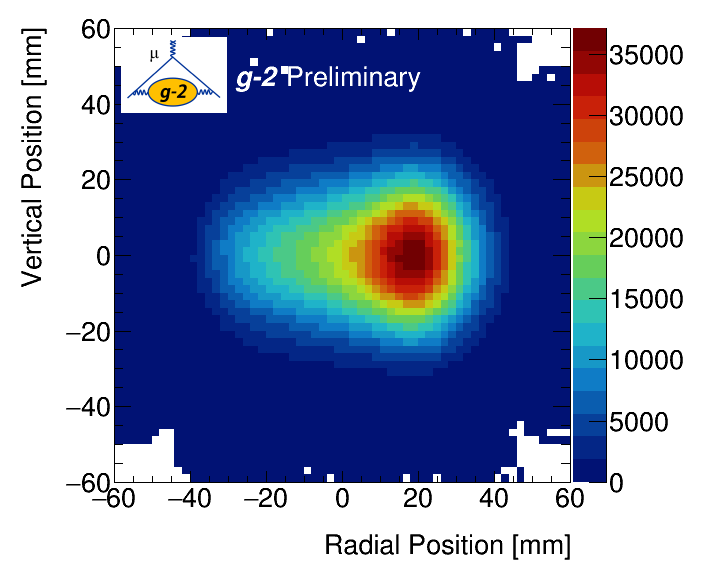
\includegraphics[width=0.7\textwidth]{BeamCrossSection}
    \caption[Extrapolated muon beam distribution cross-section]{Shown is a radial slice of the extrapolated muon distribution or beam spot. The beam is localized off center of the storage ring due to the kicker settings used, \secref{sub:kicker}. (Mention that last bit at all? Mention anything about the cuts in this plot?)}
    \label{fig:BeamCrossSection}
\end{figure}




-shown for station 12, station 18 is similar... 


    \begin{figure}[]
    \centering
        \begin{subfigure}[t]{0.47\textwidth}
            \centering
            \includegraphics[width=\textwidth]{RadialPosition}
            \caption{}
        \end{subfigure}
        \hspace{5mm}
        \begin{subfigure}[t]{0.47\textwidth}
            \centering
            \includegraphics[width=\textwidth]{VerticalPosition}
            \caption{}
        \end{subfigure}
    \caption[]{Plots courtesy of James Mott.}
    \label{fig:}
    \end{figure}


    \begin{figure}[]
    \centering
        \begin{subfigure}[t]{0.47\textwidth}
            \centering
            \includegraphics[width=\textwidth]{RadialPositionVsTime_S12}
            \caption{}
        \end{subfigure}
        \hspace{5mm}
        \begin{subfigure}[t]{0.47\textwidth}
            \centering
            \includegraphics[width=\textwidth]{VerticalPositionVsTime_S12}
            \caption{}
        \end{subfigure}
    \caption[]{Plots courtesy of James Mott.}
    \label{fig:}
    \end{figure}


    \begin{figure}[]
    \centering
        \begin{subfigure}[t]{0.47\textwidth}
            \centering
            \includegraphics[width=\textwidth]{AvgRadPosVsTime_S12}
            \caption{}
        \end{subfigure}
        \hspace{5mm}
        \begin{subfigure}[t]{0.47\textwidth}
            \centering
            \includegraphics[width=\textwidth]{AvgVertPosVsTime_S12}
            \caption{}
        \end{subfigure}
    \caption[]{Plots courtesy of James Mott.}
    \label{fig:}
    \end{figure}








    % \begin{figure}[]
    % \centering
    %     \begin{subfigure}[t]{0.47\textwidth}
    %         \centering
    %         \includegraphics[width=\textwidth]{}
    %         \caption{}
    %     \end{subfigure}
    %     \hspace{5mm}
    %     \begin{subfigure}[t]{0.47\textwidth}
    %         \centering
    %         \includegraphics[width=\textwidth]{}
    %         \caption{}
    %     \end{subfigure}
    % \caption[]{}
    % \label{fig:}
    % \end{figure}




-emphasize measurements that are directly relevant to the calorimeter \wa analysis
-cbo frequency
-cbo amplitude
-have a CBO subsection alongside general results? 


\cite{cbofrequency}



\begin{figure}[]
    \centering
    \includegraphics[width=0.9\textwidth]{CBOFrequency}
    \caption[CBO frequency]{}    
    \label{fig:CBOFrequency}
\end{figure}



\begin{figure}[]
    \centering
    \includegraphics[width=0.9\textwidth]{CBOAmplitude}
    \caption[CBO amplitude]{}    
    \label{fig:CBOAmplitude}
\end{figure}



\cleardoublepage




